\documentclass[a4paper,12pt, reqno]{article}

%Paquetes
%\usepackage[marginparwidth=70pt]{geometry}
\usepackage[english]{babel}
\usepackage{graphicx}
\usepackage{amsfonts,amssymb,amsthm,amsmath,latexsym,euscript,mathrsfs,relsize,mathtools}
\usepackage{graphicx,float,multirow, hyperref}
\usepackage{multicol,vwcol}
\usepackage{enumitem}
\usepackage{cancel,marginnote}
\usepackage[usenames,dvipsnames]{xcolor}
\usepackage{physics}
\usepackage[font=scriptsize,labelfont=bf]{caption}


\usepackage{thmtools}
\usepackage[framemethod=TikZ]{mdframed}
\theoremstyle{definition}

\newtheorem{ex}{Exercise}
\newtheorem{exeralt}{Exercise}[ex]
\newenvironment{exerr}[1]{
  \renewcommand\theexeralt{#1}
  \exeralt
}{\endexeralt}

\newenvironment{solution}{\begin{proof}[Solution:]}{\end{proof}}


\DeclareMathOperator*{\argmax}{argmax}
\DeclareMathOperator*{\argmin}{argmin}
\newcommand\darrow{\rightarrow_\rightarrow}
%Commands
\newcommand{\bec}[1]{\ensuremath{\boldsymbol{#1}}}
\newcommand{\gen}{\mathrm{span}}
\newcommand{\frob}[1]{\| #1 \|_\mathrm{F}}
\newcommand{\R}{\mathbb{R}}
\newcommand{\Z}{\mathbb{Z}}
\newcommand{\Q}{\mathbb{Q}}
\newcommand{\T}{\mathscr{T}}
\newcommand{\A}{\mathscr{A}}
\renewcommand{\S}{\mathcal{S}}
\newcommand{\I}{\mathbb{I}}
\newcommand{\B}{\mathscr{B}}
\newcommand{\D}{\mathscr{D}}
\newcommand{\C}{\mathscr{C}}
\newcommand{\N}{\mathbb{N}}
\newcommand{\X}{\mathbb{X}}
\newcommand{\Y}{\mathbb{Y}}
\newcommand{\M}{\mathcal{M}}
\newcommand{\Par}{\mathcal{P}}
\def\restrict#1{\raise-.5ex\hbox{\ensuremath|}_{#1}}


\usepackage[a4paper, top=1.8cm, bottom=1.5cm, left=2cm, right=2cm]{geometry}

\title{Solutions - Topology Munkres}
\author{\small Ana Emilia de Orellana}
\date{}

\begin{document}
\maketitle

These are my solutions to selected exercises of Munkres' Topology. \textbf{Be aware that this solutions might contain errors}. If you want to send comments, suggestions, corrections of errors/typos, etc, you can email me at anaemilia.deorellana@gmail.com or make a pull request on Github \url{https://github.com/AnadeOre/munkres-topology-solutions}

\tableofcontents

\section*{Section 13: Basis for a Topology}
\addcontentsline{toc}{section}{\protect\numberline{}Section 13: Basis of a Topology}

\begin{exerr}{1}
  Let $\X$ be a topological space; let $A\subset\X$. Suppose that for each $x\in A$ there is an open set $U\ni x$ such that $U\subset A$. Show that $A$ is open in $\X$.
\end{exerr}
\begin{solution}
  Let $U = \bigcup_{x\in\X} U_{x}$, $U$ is open, $A\subset U$ and $U\subset A$. Then $A=U$ and $A$ is open.
\end{solution}

\begin{exerr}{2}
  Consider the $9$ topologies on the set $\X = \{ a,b,c \}$. Compare them.
\end{exerr}
\begin{solution}
  \begin{align*}
    \T_{1} & = \{ \X,\varnothing \}                                                         \\
    \T_{2} & = \{ \{ a,b \},\{ a\},\X,\varnothing \}                                        \\
    \T_{3} & = \{ \X,\varnothing, \{ a,b \},\{ b \},\{ b,c \} \}                            \\
    \T_{4} & = \{ \X,\varnothing, \{ b \} \}                                                \\
    \T_{5} & = \{ \X,\varnothing, \{ a \},\{ b,c \} \}                                      \\
    \T_{6} & = \{ \X,\varnothing,\{ a,b \},\{ b,c \},\{ b \},\{ c \} \}                     \\
    \T_{7} & = \{ \X, \varnothing, \{ a,b \} \}                                             \\
    \T_{8} & = \{ \X,\varnothing, \{ a,b \},\{ a \},\{ b \} \}                              \\
    \T_{9} & = \{ \X,\varnothing, \{ a \},\{ b \},\{ c \},\{ a,b \},\{ a,c \},\{ b,c \} \}.
  \end{align*}
  PHOTO
\end{solution}

\begin{exerr}{3}
  Show that the collection $\T_{c}$ given in the example is a topology on the set $\X$. Is the collection
  \begin{equation*}
    \T_{\infty} = \{ U : \X\backslash U\text{ is infinite or empty or all of }\X \},
  \end{equation*}
  a topology on $\X$?.
\end{exerr}
\begin{solution}
  \begin{equation*}
    \T_{c} = \{ U\subset\X : U^c\text{ countable or }U^c=\X \}.
  \end{equation*}
  \begin{enumerate}
    \item $\varnothing^c = \X$ and $\X^c =\varnothing$, then $\varnothing,\X\in\T_{c}$.
    \item Let $\{ U_{\alpha} \}_{\alpha\in A}\subset\T_{c}$ and let $\widetilde{A}\subset A$ such that for all $\widetilde{\alpha}\in \widetilde{A}$, $U_{\widetilde{\alpha}}^c = \X$ and for all $\alpha\in A\backslash \widetilde{A}$, $U_{\alpha}^c$ is countable. Then
          \begin{equation*}
            \Big( \bigcup_{\alpha\in A}U_{\alpha} \Big)^c = \Big( \bigcup_{\alpha\in A\backslash \widetilde{A}}U_{\alpha} \Big)^c = \bigcap_{\alpha\in A\backslash \widetilde{A}}U_{\alpha}^c,
          \end{equation*}
          the latter is countable, therefore $\cup_{\alpha\in A}U_{\alpha}\in\T_{c}$.
    \item Let $\{ U_{i} \}_{i=1}^N\subset\T_{c}$, that is, for each $i$, $U_{i}=\varnothing$ or $U_{i}^c$ is countable.
          \begin{equation*}
            \Big( \bigcap_{i=1}^N U_{i} \Big)^c = \bigcup_{i=1}^N U_{i}^c = \begin{cases}
              \X\,                  & \text{if there exists $i$ such that }U_{i}=\varnothing; \\
              \text{is countable}\, & \text{if }\forall\,i,\,U_{i}\text{ is countable.}
            \end{cases}
          \end{equation*}
  \end{enumerate}
  $\T_{\infty}$ is not a topology. In $\R$, $U_{1} = (0,\infty)$ and $U_{2}=(-\infty,0]$ are in the topology, but their union is $\R\backslash\{ 0 \}$ which is not infinite.
\end{solution}

\begin{exerr}{4}\hfill
  \begin{enumerate}[label = (\alph*)]
    \item If $\{ \T_{\alpha} \}_{\alpha}$ is a family of topologies on $\X$, show that $\bigcap_{\alpha}\T_{\alpha}$ is a topology on $\X$. Is $\bigcup_{\alpha}\T_{\alpha}$ a topology on $\X$?
    \item Let $\{ \T_{\alpha} \}_{\alpha}$ be a family of topologies on $\X$. Show that there is a unique smallest topology on $\X$ containing all the collections $\T_{\alpha}$, and a unique largest topology contained in all $\T_{\alpha}$.
  \end{enumerate}
\end{exerr}
\begin{solution}\hfill
  \begin{enumerate}[label = (\alph*)]
    \item Proving that $\bigcap_{\alpha}\T_{\alpha}$ is a topology is trivial. To see that the union of topologies is not a topology consider $\X = \{ a,b,c \}$ and the two following topologies
    \begin{align*}
      \T_{1} &= \{ \varnothing,\X,\{ a \},\{ a,b \} \}\\
      \T_{2} &= \{ \varnothing, \X, \{ c \},\{ b,c \} \}.
    \end{align*}
    Then the union is $\T = \{ \varnothing,\X,\{ a \},\{ c \},\{ b,c \},\{ b,a \} \}$ and is not a topology because $\{ b,c \}\cap\{ b,a \} = \{ b \}\notin\T$.
    \item The smallest topology that contains all the $\T_{\alpha}$ is $\bigcap\{ \T~\text{topology} : \bigcup_{\alpha}\T_{\alpha}\subset\T \},$ and the largest topology that is contained in each $\T_{\alpha}$ is $\bigcup_{\alpha}\T_{\alpha}$.
    \item The smallest topology that contains $\T_{1}$ and $\T_{2}$ is $\T = \{ \varnothing,\X,\{ a \},\{ b \},\{ a,b \},\{ b,c \} \}$ and the greatest topology contained in $\T_{1}$ and $\T_{2}$ is $\T =\{ \varnothing,\X,\{ a \} \}$.
  \end{enumerate}
\end{solution}

\begin{exerr}{5}
  Show that if $\A$ is a basis for a topology on $\X$, then the topology generated by $\A$ equals the intersection of all topologies on $\X$ that contain $\A$. Prove the same if $\A$ is a subbasis.
\end{exerr}
\begin{solution}
  Let $(\X,\T')$ be a topological space, $\A$ basis of $\T'$ and define:
  \begin{align*}
    \T_{\A} & = \{ U : \forall\,x\in U\,\exists \,A\in\A : x\in A\subset U \} \\
    \T      & = \bigcap\{ \T : \A\subset\T \}.
  \end{align*}

  As $\A\subset\T_{\A}$, $\T\subset\T_{\A}$.

  Given $U\in\T_{\A}$, for each $x\in U$ there exists $A_{x}\in\A$ such that $x\in A_{x}\subset U$, then $U = \cup_{x\in U}A_{x}\in \A$. Therefore, $U\in \T$ and $\T_{\A}\subset\T$. With this we have $\T=\T_{\A}$.\\

  If $\A$ is a subbasis, define
  \begin{align*}
    \T_{\A} & = \{ \text{unions of finite intersections of elements in $\A$} \} \\
    \T      & = \bigcap \{ \T : \A\subset\T  \}.
  \end{align*}

  Given that $\A\subset\T_{\A}$ we have $\T\subset\T_{\A}$ and given $U\in\T_{\A}$, $U$ is union of finite intersections of elements in $\A$. Then $U\in\T$ and $\T_{\A}\subset\T$.
\end{solution}

\begin{exerr}{6}
  Show that the topologies $\R_{\ell}$ and $\R_{K}$ are not comparable.
\end{exerr}
\begin{solution}
  Let $\T_{\ell} = \T\big( \{ [a,b) : a<b \} \big)$ and $\T_{K} = \T\big( \{ (a,b) : a<b \}\cup\{ (a,b)\backslash K \} \big)$, with $K = \{ 1/n : n\in\N \}$.

  Given $x\in\R$, $[x,b)\in\T_{\ell}$ is a neighbourhood of $x$, but there does not exist a neighbourhood of $x$, $B$ in $\T_{K}$ such that $x\in B\subset [x,b)$.

  Consider now the element $B=(0,1)\backslash K$ in the basis of $\T''$ and take $0\in B$. There does not exist any interval of the form $[a,b)$ that contains $0$ and contained in $B$.
\end{solution}

\begin{exerr}{7}
  Consider the following topologies on $\R$.
  \begin{align*}
    \T_{1} & = \text{ the standard topology},                  \\
    \T_{2} & = \text{ the topology of $\R_K$},                 \\
    \T_{3} & = \text{ the finite complement topology},         \\
    \T_{4} & = \text{ the upper limit topology},               \\
    \T_{5} & = \text{ the topology having left rays as basis}.
  \end{align*}

  Determine, for each of these topologies, which of the others it contains.
\end{exerr}
\begin{solution}\hfill
  \begin{itemize}
    \item[$\T_{1}\subset\T_{4}$] Trivial.
    \item[$\T_{5}\subset\T_{1}$] Given $x\in (-\infty,b)\in\T_{5}$ there exists $(a,b)\in\T_{1}$ such that $\in(a,b)\subset(-\infty,b)$. But $\not\supset$ because given $x\in(a,b)$ $\not\exists$ $(-\infty,c)$ such that $x\in(-\infty,c)\subset(a,b)$.
    \item[$\T_{1}\subset\T_{2}$] Trivial.
    \item[$\T_{2}\subset\T_{4}$] The problem is at $0$. Now I can take $(0,x]$ or $(x,0]$, because $K$ only takes $1/n$ with $n\in\N$.
    \item[$\T_{3}\subset\T_{1}$] If $B\in\T_{3}$ is such that $\# B^c<\infty$ then given $x\in B$ there exists $(a,b)$ such that $x\in(a,b)\subset B$. But $\not\supset$ because given $(a,b)$, if $B\subset(a,b)$ then $(a,b)^c\subset B^c$ and then $\#(a,b)^c=\infty$.
    \item[$\T_{5}\not\subset\T_{3}$]  Because given $(-\infty,a)$, if we had $B\subset (-\infty,a)$ then $(-\infty,a)^c\subset B^c$ and $\#(-\infty,a)^c =\infty$.
    \item[$\T_{3}\not\subset\T_{5}$] If $B = \R\backslash\{ 0 \}$, given $x\in B$ there does not exist $(-\infty,a)\in\T_{5}$ such that $x\in(-\infty,a)\subset B$.
  \end{itemize}
\end{solution}

\begin{exerr}{8}\hfill
  \begin{enumerate}
    \item Apply Lemma 13.2 to show that the countable collection
          \begin{equation*}
            \B = \{ (a,b) : a<b,a,b\in\Q \},
          \end{equation*}
          is a basis that generates the standard topology on $\R$.
    \item Show that the collection
          \begin{equation*}
            \C = \{ [a,b) : a<b, a,b\in\Q \},
          \end{equation*}
          is a basis that generates a topology different from the lower limit topology on $\R$.
  \end{enumerate}
\end{exerr}
\begin{solution}\hfill
  \begin{enumerate}
    \item Let $x\in(a,b)\subset\R$, there exist $p,q\in\Q$ such that $a<p<x<q<b$, then $x\in(p,q)\subset (a,b)$ and then $\B$ is basis of $\T$.
    \item Taking $[\pi,4)$ and $x=\pi$, there doesn't exist $[p,q)\in\C$ such that $x\in[p,q)\subset[\pi,4)$.
  \end{enumerate}
\end{solution}

\section*{Section 16: The Subspace Topology}
\addcontentsline{toc}{section}{\protect\numberline{}Section 16: The Subspace Topology}

\begin{exerr}{1}
  Show that if $\Y$ is a subspace of $\X$ and $A\subset\Y$ then the topology $A$ inherits a subspace of $\Y$ is the same as the topology it inherits as a subspace of $\X$.
\end{exerr}
\begin{solution}
  Call $\T_{\X}, \T_{\Y}$ the topology on $\X$ and the topology on $\Y$ inherited from $\X$, that is, $\T_{\Y}= \{ \Y\cap U : U\in\T_{\X} \}$. Also, define
  \begin{align*}
    \T_{A}^\X & = \{ A\cap U : U\in\T_{\X} \}  \\
    \T_{A}^\Y & = \{ A\cap U : U\in\T_{\Y} \},
  \end{align*}
  the topologies on $A$ inherited from $\X$ and $\Y$ respectively.

  Let $V\in\T_{A}^\X$, $V = A\cup U$ with $U\in\T_{\X}$, also, $A = A\cap\Y$, then $V = (A\cap \Y)\cap U = A\cap(\Y\cap U)$, given that $\Y\cap U\in\T_{\Y}$ then $V\in\T_{A}^\Y$.

  Let $V\in\T_{A}^\Y$, $V = A\cap U$ with $U\in\T_{\Y}$, then $U = \Y\cap O$ with $O\in\T_{\X}$, then
  \begin{equation*}
    V = A\cap U = A\cap (\Y\cap O) = (A\cap \Y)\cap O = A\cap O,
  \end{equation*}
  then $V\in\T_{\X}$.
\end{solution}

\begin{exerr}{2}
  If $\T_{\X}$ and $\T'_{\X}$ are topologies on $\X$ and $\T'_{\X}$ is strictly finer that $\T_{\X}$, what can you say about the corresponding subspace topologies on the subset $\Y$ of $\X$.
\end{exerr}
\begin{solution}
  Let $V\in\T_{\Y}$ and $y\in V$, $V = \Y\cap U$ with $U\in\T_{X}$, as $\T'_{\X}\supset\T_{\X}$ given $x\in U$ there exists $U'\in\T'_{\X}$ such that $x\in U'\subset U$. Taking $V' = \Y\cap U'$ we have $y\in V'\subset V$, therefore $\T'_{\Y}\supset\T_{\Y}$.
\end{solution}

\begin{exerr}{3}
  Consider the set $\Y = [-1,1]$ as a subspace of $\R$.
  \begin{align*}
    A & = (1/2,1)\rightarrow~\text{Open in $R$ and $\Y$}.                \\
    B & = (1/2,1]\rightarrow~\text{It is $(1/2,2)\cap\Y$, open in $\Y$}. \\
    C & = [1/2,1)\rightarrow~\text{Not open, it has $1/2$ as border}.    \\
    D & = [1/2,1]\rightarrow~\text{Not open, it has $1/2$ as border}.    \\
    E & = \{ x : 0<|x|<1, 1/x\notin\N \}\rightarrow~\text{Open in $\R$.}
  \end{align*}
\end{exerr}

\begin{exerr}{4}
  A map $f:\X\to\Y$ is said to be an open map if for every open set $U$ of $\X$, the set $f(U)$ is open in $\Y$. Show that $\pi_{1}:\X\times\Y\to\X$ and $\pi_{2}:\X\times\Y\to\Y$ are open maps.
\end{exerr}
\begin{solution}
  It suffices to prove it for the basis elements. Let $A = U\times V$ with $U\in\T_{\X}$, $V\in\T_{\Y}$.
  $\pi_{1}(A) = U\in\T_{\X}$ and $\pi_{2}(A) = V\in\T_{\Y}$.

  If $A\in\T_{\X\times\Y}$, $A = \cup_{\alpha}(U_{\alpha}\times V_{\alpha}) = \big( \cup_{\alpha}U_{\alpha} \big)\times\big( \cup_{\alpha}V_{\alpha} \big)$. Then $\pi_{1}(A) = \cup_{\alpha} U_{\alpha}\in\T_{\X}$ and $\pi_{2}(A) = \cup_{\alpha}V_{\alpha}\in\T_{\Y}$
\end{solution}

\begin{exerr}{7}
  Let $\X$ be an ordered set. If $\Y$ is a proper subset of $\X$ that is convex in $\X$, does it follow that $\Y$ is an interval or a ray in $\X$?
\end{exerr}
\begin{solution}
  Not necessarily, if $\X = \Q$ and $\Y = (-\pi,\pi)\cap\Q$ there doesn't exist $a,b\in\Q$ such that $(-\pi,\pi)\cap\Q = (a,b)$.
\end{solution}

\begin{exerr}{8}
  If $L$ is a straight line in the plane, describe the topology $L$ inherits as a subspace of $\R_{\ell}\times\R$ and as a subspace of $\R_{\ell}\times\R_{\ell}$. In each case it is a familiar topology.
\end{exerr}
\begin{solution}\hfill
  \begin{itemize}
    \item If $L$ is a horizontal line at height $H$ then $[a,b)\times(c,d)\cap L = \{ [x,H) : a\leq x<b \}$, then the topology is the same as $\R_{\ell}$.
    \item If $L$ is a vertical line at $H$ then $[a,b)\times(c,d)\cap L = \{ (H,x) : a<x<b \}$ then the topology is the same as in $\R$.
    \item If $L$ is inclined then
          \begin{equation*}
            [a,b)\times(c,d)\cap L = \begin{cases}
              [a,b)\text{ in $L$ ,} & \text{if }a\leq c,b\leq d;  \\
              [a,d)\text{ in $L$ ,} & \text{if }a\leq c, d\leq b; \\
              (c,b)\text{ in $L$ ,} & \text{if }c<a, b\leq d;     \\
              (c,d)\text{ in $L$ ,} & \text{if }c<a, d\leq b
            \end{cases}
          \end{equation*}
          then it is the same topology as $\R_{\ell}$.
  \end{itemize}

  As a subspace of $\R_{\ell}\times\R_{\ell}$ it is analogous in the first two cases, but if $L$ is inclined, then the topology is the one generated by closed intervals $[a,b]$.
\end{solution}

\begin{exerr}{9}
  Show that the dictionary order topology on the set $\R\times\R$ is the same as the product topology $\R_{d}\times\R$, where $\R_{d}$ denotes $\R$ in the discrete topology. Compare this topology with the standard topology on $\R^2$.
\end{exerr}
\begin{solution}
  Let $U\in\T_{\text{dic}}^{\R\times\R}$, $U = (a\times b, c\times d)$,
  \begin{equation*}
    U = \big( \{ a \}\times(b,\infty) \big) \cup \big( (a,b)\times\R \big)\cup \big( \{ b \}\times(-\infty,d) \big)
  \end{equation*}
  then $\T_{\text{dic}}^{\R\times\R} \subset\T_{\R_{d}\times\R}$.

  Let $U\in\T_{\R_{d}\times\R}$, $U = \{ x \}\times(a,b)\in\T_{\text{dic}}^{\R\times\R}$. Then $\T_{\text{dic}}^{\R\times\R}\subset\T_{\R_{d}\times\R}$.
\end{solution}

\section*{Section 17: Closed Sets and Limit Points}
\addcontentsline{toc}{section}{\protect\numberline{}Section 17: Closed Sets and Limit Points}

\begin{exerr}{1}
  Let $\C$ be a collection of subsets of the set $\X$. Suppose that $\varnothing$ and $\X$ are in $\C$, and that finite unions and arbitrary intersections of elements of $\C$ are in $\C$. Show that the collection
  \begin{equation*}
    \T = \{ \X\backslash C : C\in\C \},
  \end{equation*}
  is a topology on $\X$.
\end{exerr}
\begin{solution}\hfill
  \begin{enumerate}
    \item $\varnothing,\X\in\C$, then $\X\backslash\X = \varnothing$ and $\C\backslash \varnothing=\X$ are in $\T$.
    \item Let $\{ U_{\alpha} \}_{\alpha\in I}\subset\T$, $U_{\alpha} = \X\backslash C_{\alpha}$ for each $\alpha$ and for some $C_{\alpha}\in\C$.
          \begin{equation*}
            \bigcup_{\alpha\in I} U_{\alpha} = \bigcup_{\alpha\in I}\big( \X\backslash C_{\alpha} \big) = \Big( \bigcap_{\alpha\in I}C_{\alpha}  \Big)^c.
          \end{equation*}

          Given that $\cap_{\alpha\in I}C_{\alpha}\in\C$ then $\cup_{\alpha\in I}U_{\alpha}\in\T$.
    \item Let $\{ U_{i} \}_{i=1}^N\subset\T$, $U_{i} = \X\backslash C_{i}$ for each $i$ with $C_{i}\in\C$.
          \begin{equation*}
            \bigcap_{i=1}^N U_{i} = \bigcap_{i=1}^N \big( \X\backslash C_{i} \big) = \Big( \bigcup_{i=1}^N C_{i}\Big)^c.
          \end{equation*}

          Given that $\cup_{i=1}^N C_{i}\in\C$, then $\cap_{i=1}^N U_{i}\in\T$.
  \end{enumerate}
\end{solution}

\begin{exerr}{2}
  Show that if $A$ is closed in $\Y$ and $\Y$ is closed in $\X$, then $A$ is closed in $\X$.
\end{exerr}
\begin{solution}
  $A$ is closed in $\Y$, then $A = F\cap\Y$ with $F$ closed in $\X$, $\Y$ closed in $\X$ then $\X\backslash\Y = U$ is open in $\X$. With this
  \begin{equation*}
    \X\backslash A = \X\backslash\big( F\cap\Y \big) = \big( \X\backslash F \big)\cup\big( \X\backslash\Y \big) = V\cup U \in\T,
  \end{equation*}
  and $A$ is closed in $\X$.
\end{solution}

\begin{exerr}{3}
  Show that if $A$ is closed in $\X$ and $B$ is closed in $\Y$, then $A\times B$ is closed in $\X\times\Y$.
\end{exerr}
\begin{solution}
  $A$ and $B$ are closed, then $\X\backslash A = U$ and $\Y\backslash B=V$ are open sets in $\X$ and $\Y$ respectively. Then
  \begin{equation*}
    (\X\times\Y)\backslash(A\times B) = U\times V,
  \end{equation*}
  proving the result.
\end{solution}

\begin{exerr}{4}
  Show that if $U$ is open in $\X$ and $A$ is closed in $\X$, then $U\backslash A$ is open in $\X$ and $A\backslash U$ is closed in $\X$.
\end{exerr}
\begin{solution}
  $A$ is closed in $\X$, then $\X\backslash A = V$ open in $\X$. Then we have
  \begin{equation*}
    U\backslash A = U\cap A^c = U\cap V
  \end{equation*}
  that is open in $\X$. And
  \begin{align*}
    \X\backslash(A\backslash U) & = \X\cap (A\backslash U)^c = \X\cap (A\cap U^c)^c = \X\cap (A^c\cup U) = \X\cap (V\cup U) = V\cup U,
  \end{align*}
  that is open in $\X$.
\end{solution}

\begin{exerr}{5}
  Let $\X$ be an ordered set in the order topology $\T_{<\,}$. Show that $\overline{(a,b)}\subset[a,b]$. Under what conditions does equality hold?
\end{exerr}
\begin{solution}
  $[a,b]$ is closed in $\T_{<\,}$ because $\X\backslash[a,b] = (-\infty,a)\cup(b,\infty)$ (or closed in one extreme if $\X$ has a maximum or minimum element). Given that $\overline{(a,b)} = \bigcap_{V\supset(a,b) \text{ closed}}V$ and $(a,b)\subset[a,b]$ we have $\overline{(a,b)}\subset[a,b]$.

  It will be $\overline{(a,b)} = [a,b]$ if for every $\delta>0$, $(a-\delta,a+\delta)\cap (a,b)\neq \varnothing$, for this to happen $a$ must have infinite successors.
\end{solution}

\begin{exerr}{6}
  Let $A,B$ and $A_{\alpha}$ denote subsets of a space $\X$. Prove the following:
  \begin{enumerate}[label=(\alph*)]
    \item If $A\subset B$, then $\overline{A}\subset \overline{B}$.
    \item $\overline{A\cup B} = \overline{A}\cup \overline{B}$.
    \item $\overline{\bigcup_{\alpha}A_{\alpha}}\supset\bigcup_{\alpha}\overline{A}_{\alpha}$; give an example where equality fails.
  \end{enumerate}
\end{exerr}
\begin{solution}\hfill
  \begin{enumerate}[label=(\alph*)]
    \item Let $A\subset B$, then
          \begin{equation*}
            \{ V\subset\X \text{ cerrado tal que }A\subset V \}\subset\{ V\subset\X \text{ cerrado tal que }B\subset V \},
          \end{equation*}
          because if $V$ is a closed set, if $B\subset V$ then $A\subset V$. Therefore, $\overline{A}\subset \overline{B}$.
    \item Let's first prove $\subset$, Let $F,G$ be closed sets in $\X$ such that $F\supset A$ and $G\supset B$. Then $A\cup B\subset G\cup F$ (finite union of closed sets is closed) and $\overline{(A\cup B)}\subset \overline{A}\cup \overline{B}$.

          To prove $\supset$ let $H$ be a closed set in $\X$ such that $H\supset (A\cup B)$, then $H\supset A$ and $H\supset B$, therefore, $\overline{A}\cup \overline{B}\subset \overline{(A\cup B)}$.
    \item Let $F$ be a closed set in $\X$ such that $F\supset\cup_{\alpha}A_{\alpha}$, then $F\supset A_{\alpha}$ for each $\alpha$ and therefore $\cup_{\alpha}\overline{A}_{\alpha}\subset \overline{\bigcup_{\alpha}A_{\alpha}}$.

          To see that the other inclusion fails consider $A_{n} = \R\backslash[-1/n,1/n]$, then $\bigcup_{n\in \N}\overline{A}_{n} = \R\backslash\{ 0 \}$ and $\overline{\bigcup A_{n}} = \overline{\R\backslash\{ 0 \}} = \R$.
  \end{enumerate}
\end{solution}

\begin{exerr}{7}
  Criticize the following ``proof'' that $\overline{\bigcup_{\alpha}A_{\alpha}}\subset\bigcup \overline{A}_{\alpha}$: If $\{ A_{\alpha} \}$ is a collection of sets in $\X$ and if $x\in\overline{\bigcup_{\alpha}A_{\alpha}}$, then every neighbourhood $U$ of $x$ intersects $\bigcup_{\alpha}A_{\alpha}$. Thus $U$ must intersect some $A_{\alpha}$, so that $x$ must belong to the closure of some $A_{\alpha}$. Therefore, $x\in\bigcup_{\alpha}A_{\alpha}$.
\end{exerr}
\begin{solution}
  The neighbourhood $U$ of $x$ intersects some $A_{\alpha}$, but different neighbourhoods could intersect different $A_{\alpha}$.
\end{solution}

\begin{exerr}{8}
  Let $A,B$ and $A_{\alpha}$ denote subspace of a space $\X$. Determine whether the following equations hold; if an equality fails, determine whether one of the inclusions $\supset$ or $\subset$ holds.
  \begin{enumerate}[label=(\alph*)]
    \item $\overline{A\cap B} = \overline{A}\cap \overline{B}$.
    \item $\overline{\bigcap_{\alpha}A_{\alpha}} = \bigcap_{\alpha}\overline{A}_{\alpha}$.
    \item $\overline{A\backslash B} = \overline{A}\backslash \overline{B}$.
  \end{enumerate}
\end{exerr}

\begin{solution}\hfill
  \begin{enumerate}[label=(\alph*)]
    \item Let $F,G$ be closed sets such that $F\supset A$ and $G\supset B$, then $(A\cap B)\subset(F\cap G)$, as the intersection of closed sets is closed, $F\cap G$ is closed, therefore $\overline{A\cap B} \subset \overline{A}\cap \overline{B}$.

          To see that $\supset$ does not hold take $A = \{ 1/n : n\in\N  \}$ and $B = \{ -1/n : n\in\N \}$, then $\overline{A} = \{ 0 \}$ and $\overline{B} = \{ 0 \}$. $A\cap B = \varnothing$, then $\overline{A\cap B} = \varnothing$ but $\overline{A}\cap \overline{B} = \{ 0 \}$.
    \item The inclusion $\supset$ does not hold for the same reason the previous one didn't. To prove $\subset$ let $F_{\alpha}$ be closed sets in $\X$ such that $A_{\alpha}\subset F_{\alpha}$. Then $\cap_{\alpha}A_{\alpha}\subset\cap_{\alpha}F_{\alpha}$ and the arbitrary intersection of closed sets is a closed set. Therefore, $\overline{\bigcap_{\alpha}A_{\alpha}} \subset \bigcap_{\alpha}\overline{A}_{\alpha}$.
    \item The inclusion $\subset$ does not hold, to see this let $A = \{ 1/n : n\in\N \}$, $B =\{ 0 \}$, then $\overline{A} = \{ 0 \} = \overline{B}$. $\overline{A}\backslash \overline{B} = \varnothing$ and $\overline{A\backslash B} = \overline{A} = \{ 0 \}$.

          To prove $\supset$ let $x\in \overline{A}\backslash \overline{B}$, then every neighbourhood $U$ of $x$ intersects $A$, but there exists $V$ neighbourhood of $x$ such that $V\cap B=\varnothing$.
          \begin{equation*}
            (V\cap U)\cap(A\backslash B) \neq \varnothing,
          \end{equation*}
          therefore $x\in \overline{A\backslash B}$
  \end{enumerate}
\end{solution}

\begin{exerr}{10}
  Show that every order topology is Hausdorff.
\end{exerr}
\begin{solution}
  Let $x,y\in\X$, $x\neq y$. Assume without any loss of generality that $x<y$. We have the following cases:
  \begin{itemize}
    \item If there exists $z$ such that $x<z<y$ then $x\in(-\infty,z)$, $y\in (z,\infty)$ and $(-\infty,z)\cap(z,\infty) = \varnothing$.
    \item If there is no such $z$ then $y = x+1$ (the immediate successor), $x\in(-\infty,y)$, $y\in(x,\infty)$ and $(-\infty,y)\cap(x,\infty) = \varnothing$.
  \end{itemize}
\end{solution}

\begin{exerr}{11}
  Show that the product of two Hausdorff spaces is Hausdorff
\end{exerr}
\begin{solution}
  We know that the basis of $\T_{\X\times\Y}$ is
  \begin{equation*}
    \{ U\times V : U\in\T_{\X},V\in\T_{\Y} \}.
  \end{equation*}

  Let $a\times b, c\times d\in\X\times\Y$, $a\times b\neq c\times d$.
  \begin{itemize}
    \item If $a\neq c$ and $b\neq d$ then there exist $U_{a},U_{c}\in\T_{\X}$, $V_{b},V_{d}\in\T_{\Y}$ neighbourhoods of $a,b,c,d$ such that $U_{a}\cap U_{c}=\varnothing$, and $V_{b}\cap V_{d}=\varnothing$. Then $a\times b\in U_{a}\times V_{b}$, $c\times d\in U_{c}\times V_{d}$ and
          \begin{equation*}
            (U_{a}\times V_{b})\cap (U_{c}\times V_{d}) = (U_{a}\cap U_{c})\times (V_{c}\cap V_{d}) = \varnothing.
          \end{equation*}
    \item If $a=c$, $b\neq d$, let $U$ be a neighbourhood of $a$ and $c$, $V_{b},V_{d}$ disjoint neighbourhoods of $b$ and $d$. Then $a\times b\in U\times V_{b}$, $c\times d\in U\times V_{d}$ and
          \begin{equation*}
            (U\times V_{b})\cap (U\times V_{d}) = U\times (V_{b}\cap V_{d}) = U\times \varnothing = \varnothing.
          \end{equation*}
  \end{itemize}
\end{solution}

\begin{exerr}{12}
  Show that a subspace of a Hausdorff space is Hausdorff.
\end{exerr}
\begin{solution}
  Let $(\X,\T_{\X})$ be a Hausdorff space, $(\Y,\T_{\Y})$ subspace of $\X$. Let $x,y\in\Y$, $x\neq y$. As $\X$ is Hausdorff, there exist disjoint neighbourhoods $U,V\in\T_{\X}$ of $x$ and $y$. Clearly $x\in U\cap\Y$, $y\in V\cap\Y$, $U\cap\Y, V\cap\Y\in\T_{\Y}$ and
  \begin{equation*}
    (U\cap\Y)\cap (V\cap\Y) = (U\cap V)\cap \Y = \varnothing\cap\Y = \varnothing.
  \end{equation*}
\end{solution}

\begin{exerr}{13}
  Show that $\X$ is Hausdorff if and only if the diagonal $\Delta = \{ x\times x : x\in\X \}$ is closed in $\X\times\X$.
\end{exerr}
\begin{solution}\hfill
  \begin{itemize}
    \item[($\Longrightarrow$)] Let's see that $\Delta = \overline{\Delta}$. Obviously $\Delta\subset \overline{\Delta}$, suppose by contradiction that $\overline{\Delta}\not\subset\Delta$. Let $x\times y\in\overline{\Delta}$, $x\neq y$. Given $z\in\X$, consider the two following options:
      \begin{itemize}
        \item If $z\neq x$ there exist (because $\X$ is Hausdorff) disjoint neighbourhoods $U,V$ of $x$ and $z$.
        \item If $z\neq y$ then there exist disjoint neighbouthoods $\widetilde{U},\widetilde{V}$ of $y$ and $z$.
      \end{itemize}
      Therefore, for any $z\times z\in\X\times\X$ there exists a neighbourhood $U\times \widetilde{U}$ of $x\times y$ such that $U\times \widetilde{U}\cap\Delta = \varnothing$. Then $x\times y\notin \overline{\Delta}$, which contradicts our assumption.
    \item[($\Longleftarrow$)] $\Delta$ is closed in $\X\times\X$, then $\Delta = \overline{\Delta}$. Let $x,y\in\X$, $x\neq y$. There must exist $U,V$ neighbourhoods of $x$ and $y$ such that $U\cap V = \varnothing$, because if there existed $z\in U\cap V$ then $U\times V$ would be a neighbourhood of $z\times z$ and then $x\times y\in\overline{\Delta}$, which cannot happen.
  \end{itemize}
\end{solution}

\begin{exerr}{14}
  In the finite complement topology, $\T_{c}$ on $\R$, to what point or points does the sequence $x_{n}=1/n$ converge?.
\end{exerr}
\begin{solution}
  $\R$ with the finite complement topology is not Hausdorff, therefore, convergent sequence do not have a unique limit.

  Suppose that $\{ 1/n \}$ converges to some $x_{0}\in\R$. Then for every $U\in \T_{c}$, $U\ni x_{0}$, there exists $N\in\N$ such that $1/n\in U$ for every $n\geq N$. Because $U$ is open, then $U^c$ is finite. Suppose $U^c\supset\{ 1/n : N_{0}\leq n< N_{1} \}$ then for every $n\geq N_{1}$, $U\supset\{ 1/n \}$. Therefore, every open set in $\T_{c}$ contain infinite elements of the sequence, so $\{ 1/n \}$ converges to every point.
\end{solution}

\begin{exerr}{15}
  Show the $T_{1}$ axiom is equivalent to the condition that for each pair of points of $\X$, each has a neighbourhood not containing the other.
\end{exerr}
\begin{solution}\hfill
  \begin{itemize}
    \item[($\Longrightarrow$)] $\{ x \}$ is closed for every $x\in\X$, then given $x,y\in\X$, the sets $V = \X\backslash\{ x \}$, $U = \X\backslash\{ y \}$ are disjoint neighbourhoods of $y$ and $x$ such that $x\notin V$ and $y\notin U$.
    \item[($\Longleftarrow$)] For every $x\neq y$ there exist $U_{x},V_{y}$ neighbourhoods of $x$ and $y$ such that $x\notin V_{y}$ and $y\notin U_{x}$. Given $x_{0}\in\X$, define $O = \cup_{y\neq x_{0}}V_{y}$, $O$ is open and $\X\backslash{x_{0}} = O$, then $\{ x_{0} \}$ is closed.
  \end{itemize}
\end{solution}

\begin{exerr}{16}
  Consider the five topologies on $\R$:
  \begin{align*}
    \T_{1} & = \text{ the standard topology},                  \\
    \T_{2} & = \text{ the topology of $\R_K$},                 \\
    \T_{3} & = \text{ the finite complement topology},         \\
    \T_{4} & = \text{ the upper limit topology},               \\
    \T_{5} & = \text{ the topology having left rays as basis}.
  \end{align*}
  \begin{enumerate}[label = (\alph*)]
    \item Determine the closure of the set $K = \{ 1/n : n\in\N \}$ under each of these topologies.
    \item Which of these topologies satisfy the Hasudorff axiom? The $T_{1}$ axiom?
  \end{enumerate}
\end{exerr}
\begin{solution}\hfill
  \begin{enumerate}[label = (\alph*)]
    \item \hfill
          \begin{itemize}
            \item In $\T_{1}$, $\overline{K} = K\cup \{ 0 \}$.
            \item In $\T_{2}$ the open sets are of the form $(a,b)$ and $(a,b)\backslash K$. Given that the open sets $(a,b)$ contain $\{ 0 \}$ then $0\in \overline{K}$. But if $0\in (a,b)\backslash K$ then that open set does not have limit points of $K$. Therefore, in $\T_{2}$, $\overline{K} = K\cup \{ 0 \}$.
            \item In $\T_{3}$ the complements of open sets contain at most finite elements of $K$. Then every open set contains infinite elements of $K$, that is, if $U\in\T_{3}$, $U\cap K\neq \varnothing$ and $(U\backslash\{ x_{0} \})\cap K \neq \varnothing$ for any $x_{0}\in\R$. Then $\overline{K} = \R$.
            \item In $\T_{4}$ $K = \overline{K}$ because given $x_{0}\in K$,
                  \begin{itemize}
                    \item If $x_{0}\leq0$ then there exists $\delta>0$ such that $(x_{0}-\delta,x_{0}]$ is an neighbourhood of $x_{0}$ with $(x_{0}-\delta,x_{0}]\cap K =\varnothing$.
                    \item If $x_{0}>1$ then given $1<y<x_{0}$, $(y,x_{0}]$ is a neighbourhood of $x_{0}$ and $(y,x_{0}]\cap K = \varnothing$.
                  \end{itemize}
            \item In $\T_{5}$, $\overline{K} = [0,\infty)$.
                  \begin{itemize}
                    \item If $(-\infty,a)$ is a neighbourhood of $x_{0}\geq0$, it contains infinite elements of $K$.
                    \item If $x_{0}<0$ then $(-\infty,0)$ is a neighbourhood of $x_{0}$ and $(-\infty,0)\cap K = \varnothing$.
                  \end{itemize}
          \end{itemize}
    \item \hfill
          \begin{itemize}
            \item[\checkmark] $\T_{1}$ is $T_{1}$ and Hausdorff.
            \item[\checkmark] $\T_{2}$ is $T_{1}$ and Hausdorff because it includes $\T_{1}$.
            \item[\checkmark] $\T_{3}$ is $T_{1}$ and Hausdorff: singletons are closed because $\R\backslash\{ x \}$ is a set with finite complement, and therefore is open, so $\{ x \}$ is closed. $\X\backslash\{ x \}$, $\X\backslash\{ y \}$ are disjoint neighbourhoods of any two points $x\neq y$.
            \item[\checkmark] $\T_{4}$ is $T_{1}$ and Hausdorff: if $x\neq y$, suppose $x<y$ then $(x-1,x]$ is a neighbourhood of $x$, let $\varepsilon = \frac{y-x}{2}$, then $(x+\varepsilon,y]$ is a neighbourhood of $y$ and $(x-1,x]\cap (x+\varepsilon,y] = \varnothing$.
            \item[$\times$] $\T_{5}$ is not $T_{1}$, if $x\neq y$, suppose $x<y$, then every neighbourhood of $y$ contains $x$.
          \end{itemize}
  \end{enumerate}
\end{solution}

\begin{exerr}{17}
  Consider the lower limit topology on $\R$ and the topology given by the basis $\C = \{ [a,b) : a<b, a,b\in\Q \}$. Determine the closures of the intervals $A = (0,\sqrt{2})$ and $B = (\sqrt{2},3)$ in these two topologies.
\end{exerr}
\begin{solution}\hfill\\

  \noindent$\R_{\ell}$:
  \begin{itemize}
    \item[$A$:] $0\in \overline{A}$ because if $[a,b)\ni 0$ then it contains infinite elements of $A$. $\sqrt{2}\notin \overline{A}$ because $[\sqrt{2},\sqrt{2}+1)$ is a neighbourhood of $\sqrt{2}$ that does not intersect $A$.
    \item[$B$:] $\sqrt{2}\in \overline{B}$ because if $[a,b)\ni\sqrt{2}$ then it contains infinite elements of $B$. $3\notin B$ because $[3,4)$ is a neighbourhood of $3$ that does not intersect $B$.
  \end{itemize}
  $\R_{\C}$
  \begin{itemize}
    \item[$A$:] $0\in \overline{A}$ because any set $[a,b)\ni0$ with $a,b\in Q$ contains infinite elements of $A$. $\sqrt{2}\in \overline{A}$ because if $[a,b)$ is a neighbourhood of $\sqrt{2}$ then $a\in\Q$, $a<\sqrt{2}$, then the set contains infinite elements of $A$.
    \item[$B$:] $\sqrt{2}\in B$ because any neighbourhood $[a,b)\ni\sqrt{2}$ has $b\in Q$, $b>\sqrt{2}$, then it must contain infinite eleents of $B$. $3\notin B$ because $[3,4)$ is an environment of $3$ that does not intersect $B$.
  \end{itemize}
\end{solution}

\begin{exerr}{18}
  Determine the closures of the following subsets of the ordered square:
  \begin{align*}
    A & = \{ (1/n)\times 0 : n\in\N \},             \\
    B & = \{ (1-1/n)\times \frac{1}{2} : n\in\N \}, \\
    C & = \{ x\times0 : 0<x<1 \},                   \\
    D & = \{ x\times \frac{1}{2} : 0<x<1 \},        \\
    E & = \{ \frac{1}{2}\times y : 0<y<2 \}.
  \end{align*}
\end{exerr}
\begin{solution}
  \begin{equation*}
    A =  \{ (1/n)\times 0 : n\in\N \}.
  \end{equation*}
  $0\times 1$ is the limit point because its neighbourhoods are $(0\times a,b\times c)$ with $a<1$, $b>0$ and $c<1$ and that interval contains infinite elements of $A$.
  \begin{equation*}
    B = \{ (1-1/n)\times \frac{1}{2} : n\in\N \}.
  \end{equation*}
  Same as before but with $1\times 0$, its neighbourhoods are $(a\times b,1\times c)$ with $\frac{1}{2}<a,b<1$ and $c<\frac{1}{2}$.
  \begin{equation*}
    C = \{ x\times0 : 0<x<1 \}.
  \end{equation*}
  $0\times0\notin \overline{C}$ because $(0\times0,0\times \frac{1}{2})\cap C = \varnothing$. $1\times 1\notin \overline{C}$ because $(1\times \frac{1}{2},1\times 1]\cap C = \varnothing$.
  But $\{ x\times 1 : 0\leq x<1 \}\subset \overline{C}$ and $1\times 0\in \overline{C}$.
  \begin{equation*}
    D = \{ x\times \frac{1}{2} : 0<x<1 \}.
  \end{equation*}
  \begin{equation*}
    \overline{D} = \{ x\times 1 : 0\leq x<1 \}\cup\{ 0\times x : 0<x\leq 1 \}.
  \end{equation*}

  \begin{equation*}
    E = \{ \frac{1}{2}\times y : 0<y<2 \}.
  \end{equation*}
  $\frac{1}{2}\times 0\in \overline{E}$ because every neighbourhood is of the form $(a\times b, \frac{1}{2}\times c)$ with $a<\frac{1}{2}$, $b,c>0$. $\frac{1}{2}\times 1\in \overline{E}$ because every neighbourhood is of the form $(\frac{1}{2}\times a, b\times c)$, $b,c>0$, $a<1$.
\end{solution}

\begin{exerr}{19}
  If $A\subset\X$, we define the boundary of $A$ by the equation $\partial A = \overline{A}\cap\overline{(\X\backslash A)}$.
  \begin{enumerate}[label=(\alph*)]
    \item Show that $A^\circ$ and $\partial A$ are disjoint, and $\overline{A} = A^\circ\cup\partial A$.
    \item Show that $\partial A = \varnothing$ $\Longleftrightarrow$ $A$ is both open and closed.
    \item Show that $U$ is open $\Longleftrightarrow$ $\partial U = \overline{U}\backslash U$.
    \item If $U$ is open, is it true that $U = (\overline{U})^\circ$? Justify your answer.
  \end{enumerate}
\end{exerr}

\begin{solution}\hfill
  \begin{enumerate}[label=(\alph*)]
    \item Let $x\in A^\circ\cap \partial A$.
          \begin{itemize}
            \item Because $x\in A^\circ$ then $x\in V_{0}$ for some $V_{0}\in\T$, $V_{0}\subset A$.
            \item Because $x\in\partial A$ then $x\in F$ for every $F\supset(\X\backslash A)$.
          \end{itemize}
          Absurd, then $A^\circ\cap\partial A = \varnothing$.

          If $x\in \overline{A}$ then for every $U\in\T$, $U\ni x$, $U\cap A\neq \varnothing$. If $U\cap A\neq \varnothing$, then $U\not\subset A^c$ so $U\cap A^c\neq \varnothing$ and $x\in\overline{\X\backslash A}$. Also, if $U\cap A\neq \varnothing$ then $U\cap V\neq \varnothing$ with $V\in\T$, $V\in A$.

    \item Let's first prove $\Longrightarrow$. If $\partial A = \varnothing$ then $\overline{A} = A^\circ$, as $A^\circ \subset A\subset \overline{A}$ then $\overline{A} = A = A^\circ$, then $A$ is open and closed.
          Now $\Longleftarrow$. If $A$ is open then $A\in\T$, if $A$ is closed then $\X\backslash A\in\T$. Then, given $x\in\X$ there exists $U$ such that $x\in U\subset A$ or $x\in U\subset\X\backslash A$, then $x\notin \overline{A}$ and $x\notin \overline{\X\backslash A}$, so $\partial A = \varnothing$.

    \item Let's first prove $\Longrightarrow$. If $U$ is open, then
          \begin{equation*}
            \partial U = \overline{U}\cap\overline{(\X\backslash U)} = \overline{U}\cap(\X\backslash U) = \overline{U} \cap\X\cap U^c = \overline{U}\backslash U.
          \end{equation*}

          For $\Longleftarrow$, if $\partial U = \overline{U}\backslash U$ then
          \begin{equation*}
            U^\circ = (U^\circ\cup \partial U) \backslash \partial U = \overline{U}\backslash \partial U = \overline{U}\backslash(\overline{U}\backslash U ) = U.
          \end{equation*}
    \item It is not true. If $U = \R\backslash\{ 0 \}$, $U$ is open, $\overline{U} = \R$ and $U^\circ = \R$, but $U\neq (\overline{U})^\circ$.
  \end{enumerate}
\end{solution}

\begin{exerr}{20}
  Find the boundary and the interior of each of the following subsets of $\R^2$.
  \begin{enumerate}[label = (\alph*)]
    \item $A = \{ x\times y : y=0 \}$
    \item $B = \{ x\times y : x>0, y\neq 0 \}$
    \item $C = A\cup B$.
    \item $D = \{ x\times y : x\in \Q \}$
    \item $E = \{ x\times y : 0<x^2-y^2\leq 1 \}$
    \item $F = \{ x\times y : x\neq0, y\leq 1/x \}$.
  \end{enumerate}
\end{exerr}
\begin{solution}\hfill
  \begin{enumerate}[label = (\alph*)]
    \item $A = \overline{A}$, $A^\circ = \varnothing$.
    \item $B = B^\circ$, $\overline{B} = \{ x\times y : x\geq0, y\in\R \}$.
    \item $\overline{A\cup B} = A\cup B\cup \{ x\times y : x=0 \}$, $(A\cup B)^\circ = \{ x\times y : x>0 \}$.
    \item $\overline{D} = \R\times\R$, $D^\circ = \varnothing$.
    \item $\overline{E} = \{ x\times y : 0\leq x^2-y^2\leq1 \}$, $E^\circ = \{ x\times y : 0<x^2-y^2<1 \}$.
    \item $\overline{F} = \{ x\times y : x\neq0, y\leq 1/x \}\cup\{ x\times y : x=0 \}$, $F^\circ = \{ x\times y : x\neq0, y<1/x \}$.
  \end{enumerate}
\end{solution}

\section*{Section 18: Continuous Functions}
\addcontentsline{toc}{section}{\protect\numberline{}Section 18: Continuous Functions}

\begin{exerr}{2}
  Suppose that $f:\X\to\Y$ is continuous. If $x$ is a limit point of the subset $A$ of $\X$, is it necessarily true that $f(x)$ is a limit point of $f(A)$?
\end{exerr}
\begin{solution}
  No, let $f:\R\to\R$, $f(x)\equiv 8$. Let $A = [0,1)$, $x=1$ is a limit point of $A$, $f(1) =8$, $f([0,1))=8$ and $8$ is not an isolated point of $\{ 8 \}$.
\end{solution}

\begin{exerr}{3}
  Let $\X$ and $\X'$ denote a single set in two topologies $\T$ and $\T'$, respectively. Let $i:\X'\to\X$ be the identity function.
  \begin{enumerate}[label= (\alph*)]
    \item Show that $i$ is continuous $\Longleftrightarrow$ $\T\subset\T'$.
    \item Show that $i$ is a homeomorphism $\iff$ $\T' = \T$.
  \end{enumerate}
\end{exerr}
\begin{solution}\hfill
  \begin{enumerate}[label= (\alph*)]
    \item \hfill
          \begin{itemize}
            \item[($\Longrightarrow$)] $i$ is continuous, then for every $U\in\T$, $f^{-1}(U)\in\T'$, but $f^{-1}(U) = U$, then $U\in\T$ implies $U\in\T'$, so $\T\subset\T'$.
            \item[($\Longrightarrow$)] If $\T\subset\T'$ then for every $U\in\T$, $U\in\T'$. Given $U\in\T$, $f^{-1}(U) = U\in\T'$, then $i$ is continuous.
          \end{itemize}
    \item
  \end{enumerate}
\end{solution}

\begin{exerr}{4}
  Given $x_{0}\in\X$ and $y_{0}\in\Y$, show that the maps $f:\X\to\X\times\Y$ and $g:\Y\to\X\times\Y$ defined by
  \begin{equation*}
    f(x) = x\times y_{0}\quad \text{and}\quad g(y) = x_{0}\times y,
  \end{equation*}
  are imbeddings.
\end{exerr}
\begin{solution}
  To see that $f$ is an imbedding we must see that $f:\X\to f(\X)$ is a homeomorphism. $f(\X) = \X\times\{ y_{0 } \}$, given $U\times V$ open in $\X\times\{ y_{0} \}$, it must be $V = \{ y_{0} \}\cap \widetilde{V}$, then $U$ is open in $\X$ and $f^{-1}(U\times\{ y_{0} \}) = U\in\T_{\X}$.

  Likewise, if $U\in\T_{\X}$, $f(U) = U\times\{ x_{0} \}$, that is open in $\X\times\{ y_{0} \}$. Then $f$ and $f^{-1}$ are continuous, given that $f$ is bijective, it is an imbedding.

  The proof for $g$ is analogous.
\end{solution}

\begin{exerr}{5}
  Show that the subspace $(a,b)$ of $\R$ is homeomorphic with $(0,1)$ and the subspace $[a,b]$ of $\R$ is homeomorphic with $[0,1]$.
\end{exerr}
\begin{solution}
  The function $f(x) = \frac{x-a}{b-a}$ is a homeomorphism between those spaces.
\end{solution}

\begin{exerr}{7}\hfill
  \begin{enumerate}[label=(\alph*)]
    \item Suppose that $f:\R\to\R$ is ``continuous from the right'', that is,
          \begin{equation*}
            \lim_{x\to a^+}f(x) = f(a),
          \end{equation*}
          for each $a\in\R$. Show that $f$ is continuous when considered as a function from $\R_{\ell}$ to $\R$.
    \item Can you conjecture what functions $f:\R\to\R$ are continuous when considered as maps from $\R$ to $\R_{\ell}$? As maps from $\R_{\ell}$ to $\R_{\ell}$?
  \end{enumerate}
\end{exerr}
\begin{solution}\hfill
  \begin{enumerate}[label=(\alph*)]
    \item Let $\T_{\ell}$ and $\T_{s}$ be the topologies of $\R_{\ell}$ and $\R$ respectively. Because $f$ is continuous from the right then
          \begin{equation*}
            f([x_{0},x_{0}+\delta)) \subset \big( f(x_{0})-\varepsilon, f(x_{0})+\varepsilon \big).
          \end{equation*}

          Then $[x_{0},x_{0}+\delta)\subset f^{-1}\big( f(x_{0})-\varepsilon,f(x_{0})+\varepsilon \big)$. Given that $[x_{0},x_{0}+\delta)$ is open in $\T_{\ell}$ then $f$ is continuous.
    \item
  \end{enumerate}
\end{solution}

\begin{exerr}{8}
  Let $\Y$ be an ordered set in the order topology. Let $f,g:\X\to\Y$ be continuous.
  \begin{enumerate}[label=(\alph*)]
    \item Show that the set $\{ x : f(x)\leq g(x) \}$ is closed in $\X$.
    \item Let $h:\X\to\Y$ be the function
          \begin{equation*}
            h(x) = \min\{ f(x), g(x) \}.
          \end{equation*}

          Show that $h$ is continuous. [Hint: Use the pasting lemma.]
  \end{enumerate}
\end{exerr}

\begin{solution}\hfill
  \begin{enumerate}[label=(\alph*)]
    \item Let $A = \{ x : f(x)\leq g(x) \}$, we will see that $\X\backslash A$ is open. $f$ and $g$ are continuous, then for every $V\in\T_{<\,}$, $f^{-1}(V), g^{-1}(V)\in\T_{\X}$
          \begin{equation*}
            f^{-1}\big( (g(x),\infty) \big) = \{ x\in\X : f(x)\in(g(x),\infty) \} = \{ x\in\X : f(x)>g(x) \}.
          \end{equation*}

          Then $\X\backslash A$ is the preimage of $(g(x),\infty)$, which is open in $\T_{<\,}$, because $f$ is continuous, $\X\backslash A$ is open and $A$ closed.
    \item We can write the function $h$ as
          \begin{equation*}
            h(x) =\begin{cases}
              f(x) & \text{if }f(x)\leq g(x)  \\
              g(x) & \text{if }g(x)\leq f(x).
            \end{cases}
          \end{equation*}
          Also
          \begin{equation*}
            \X = A\cup B = \{ x: f(x)\leq g(x) \}\cup \{ x : g(x)\leq f(x) \},
          \end{equation*}
          the sets $A$ and $B$ are closed and $f(x) = g(x)$ if $x\in A\cap B$, then $h$ is continuous.
  \end{enumerate}
\end{solution}

\begin{exerr}{10}
  Let $f: A\to B$ and $g:C\to D$ be continuous functions. Let us define a map $f\times g: A\times C\to B\times D$ by the equation
  \begin{equation*}
    (f\times g)(a\times c) = f(a)\times g(c).
  \end{equation*}

  Show that $f\times g$ is continuous.
\end{exerr}
\begin{solution}
  Let $U\times V$ be an open set in $B\times D$,
  \begin{equation*}
    (f\times g)^{-1}(U\times V) = f^{-1}(U)\times g^{-1}(V).
  \end{equation*}

  Given that $f$ and $g$ are continuous then $f^{-1}(U)$ and $g^{-1}(V)$ are open sets in $A$ and $C$ respectively, and $f^{-1}(U)\times f^{-1}(V)$ is open in $A\times C$.
\end{solution}

\begin{exerr}{13}
  Let $A\subset\X$, let $f:A\to\Y$ be continuous, let $\Y$ be Hausdorff. Show that if $f$ may be extended to a continuous function $g:\widetilde{A}\to\Y$, then $g$ is uniquely determined by $f$.
\end{exerr}
\begin{solution}
  Let $x\in A'$, for every neighbourhood $U$ of $x$, $U\cap\big( A\backslash\{ x \} \big) \neq \varnothing$. Suppose $g(x)\neq \widetilde{g}(x)$. Because $\Y$ is Hausdorff there exist $V$ and $\widetilde{V}$, neighbourhoods of $g(x)$ and $\widetilde{g}(x)$ such that $V\cap \widetilde{V} = \varnothing$.

  $g^{-1}(V)$ and $\widetilde{g}^{-1}(\widetilde{V})$ are neighbourhoods of $x$ in $\X$, then it also is $g^{-1}(V)\cap \widetilde{g}^{-1}(\widetilde{V})$, and as $x\in A'$ then
  \begin{equation*}
    (g^{-1}(V)\cap \widetilde{g}^{-1}(\widetilde{V}))\cap\big( A\backslash\{ x \} \big)\neq \varnothing.
  \end{equation*}
  But in $A$, $g = \widetilde{g}$, then there exists $y\in g^{-1}(V)\cap g^{-1}(\widetilde{V})\cap(A\backslash\{ x \})$ and $g^{-1}(V)\cap \widetilde{g}^{-1}(\widetilde{V}) = g^{-1}(V\cap \widetilde{V})$.

  Then $y\in g^{-1}(V\cap \widetilde{V})$, but $V\cap \widetilde{V} =\varnothing$, absurd. The absurd follows from assuming that $\widetilde{g} = g$ in $A'$.
\end{solution}

\section*{Section 19: The Product Topology}
\addcontentsline{toc}{section}{\protect\numberline{}Section 19: The Product Topology}

\begin{exerr}{1}
  Prove Theorem 19.2: Let $\{ (\X_{\alpha},\T_{\alpha}) \}_{\alpha\in J}$ be a sequence of topological spaces such that each $\T_{\alpha}$ is generated by the basis $\B_{\alpha}$. The collection $B$ of all sets of the form $\prod_{\alpha\in J}B_{\alpha}$, where $B_{\alpha}\in\B_{\alpha}$ for each $\alpha$ is a basis for the $\T_{\text{box}}$ in $\prod_{\alpha\in J}\X_{\alpha}$.
\end{exerr}
\begin{solution}
  We need to see that the two properties for a basis are satisfied.
  \begin{enumerate}
    \item Let $(x_{\alpha})_{\alpha\in J}\in\prod_{\alpha\in J}\X_{\alpha}$. Given that $\T_{\alpha}$ is generated by $\B_{\alpha}$ then there exists $B_{\alpha}\in\B_{\alpha}$ such that $B_{\alpha}\ni x_{\alpha}$. Doing this for each $\alpha$ yields that $(x_{\alpha})_{\alpha\in J}\in\prod_{\alpha\in J}B_{\alpha}\in B$.
    \item Let $(x_{\alpha})_{\alpha\in J}\in \Big( \prod_{\alpha\in J}B_{\alpha} \Big)\cap \Big( \prod_{\gamma\in J}B_{\gamma} \Big)$. This intersection also belongs to $B$, so the property is trivial.
  \end{enumerate}
\end{solution}

\begin{exerr}{2}
  Prove Theorem 19.3: Let $A_{\alpha}$ be a subspace of $\X_{\alpha}$, for each $\alpha\in J$. Then $\prod_{\alpha}A_{\alpha}$ is a subspace of $\prod_{\alpha}\X_{\alpha}$ if both products are given the box topology or if both products are given the product topology.
\end{exerr}
\begin{solution}\hfill\\

  \noindent\textbf{Box Topology:} Let $\T_{\text{box}}$ be the box topology in $\prod_{\alpha\in J}A_{\alpha}$, that is, the topology generated by $\prod_{\alpha\in J}U_{\alpha}$ with $U_{\alpha}=V_{\alpha}\cap A_{\alpha}$, $V_{\alpha}$ open in $\X_{\alpha}$.
  \begin{equation*}
    \prod_{\alpha\in J}U_{\alpha} = \prod_{\alpha\in J}(V_{\alpha}\cap A_{\alpha}) = \Big( \prod_{\alpha\in J}V_{\alpha} \Big)\cap \Big( \prod_{\alpha\in J}A_{\alpha} \Big).
  \end{equation*}

  \noindent\textbf{Product Topology:} Let $\T_{\text{prod}}$ be the product topology in $\prod_{\alpha\in J}A_{\alpha}$. Let $\prod_{\alpha\in J}U_{\alpha}\in\T_{\text{prod}}$, that is, there are finite $U_{\alpha}$ such that $U_{\alpha_j} = V_{\alpha_{j}}\cap A_{\alpha_{j}}$ and the rest are $A_{\alpha_{i}}$, then
  \begin{equation*}
    \prod_{\alpha\in J} U_{\alpha} = \prod_{\alpha_{j}}(V_{\alpha_{j}}\cap A_{\alpha_{j}})\times \prod_{\alpha_{i}}A_{\alpha_{i}} = \Big( \prod_{\alpha_{j}}V_{\alpha_{j}}\times\prod_{\alpha_{i}}\X_{\alpha_{i}} \Big)\cap \Big( \prod_{\alpha}A_{\alpha} \Big).
  \end{equation*}
\end{solution}

\begin{exerr}{3}
  Prove Theorem 19.4: If each space $\X_{\alpha}$ is a Hausdorff space, then $\prod_{\alpha\in J}\X_{\alpha}$ is a Hausdorff space in both the box and product topologies.
\end{exerr}
\begin{solution}
  Let $(x_{\alpha})_{\alpha\in J}, (y_{\alpha})_{\alpha\in J}\in\prod_{\alpha}\X_{\alpha}$, suppose without any loss of generality that $x_{\alpha}\neq y_{\alpha}$ for every $\alpha$. Given that for each $\alpha$, $\X_{\alpha}$ is a Hausdorff space there exists for every $\alpha$ disjoint sets $U_{\alpha}, V_{\alpha}$ such that $U_{\alpha}\ni x_{\alpha}$ and $V_{\alpha}\ni y_{\alpha}$.

  \noindent\textbf{Box Topology:} $\prod_{\alpha\in J}U_{\alpha}$, and $\prod_{\alpha\in J} V_{\alpha}$ are envirnonments of $(x_{\alpha})_{\alpha}$ and $(y_{\alpha})_{\alpha}$ and
  \begin{equation*}
    \Big( \prod_{\alpha}U_{\alpha} \Big)\cap \Big( \prod_{\alpha}V_{\alpha} \Big) = \prod_{\alpha\in J} (U_{\alpha}\cap V_{\alpha}) = \varnothing.
  \end{equation*}

  \noindent\textbf{Product Topology:} $\pi_{\alpha}^{-1}(U_{\alpha}) = \prod_{\beta\in J}O_{\beta}$, with $O_{\beta} = U_{\alpha}$ if $\alpha = \beta$ or $\X_{\beta}$ if $\beta\neq \alpha$. Likewise, $\pi_{\alpha}^{-1}(V_{\alpha}) = \prod_{\beta\in J}P_{\beta}$.
  $\prod_{\beta\in J}O_{\beta}$ is a neighbourhood of $(x_{\alpha})_{\alpha}$ and $\prod_{\beta\in J}P_{\beta}$ is a neighbourhood of $(y_{\alpha})_{\alpha\in J}$ and they are disjoint.
\end{solution}

\begin{exerr}{4}
  Show that $(\X_{1}\times\cdots\times\X_{n-1})\times \X_{n}$ is homeomorphic with $\X_{1}\times\cdots\times\X_{n}$.
\end{exerr}
\begin{solution}
  Let $f: (\X_{1}\times\cdots\times\X_{n-1})\times \X_{n}\to \X_{1}\times\cdots\times\X_{n}$, be the mapping $(x_{1},\dots,x_{n-1})\times x_{n}\mapsto x_{1}\times\cdots \times x_{n}$.
  The function $f$ is clearly a homeomorphism.
\end{solution}

\begin{exerr}{5}
  One of the implications stated in Theorem 19.6 holds for the box topology. Which one?
\end{exerr}
\begin{solution}
  In the box topology, if $f:A\to\prod_{\alpha\in J}\X_{\alpha}$, $f(a) = (f_{\alpha}(a))$ is continuous, then each $f_{\alpha}$ is continuous. This is because the projection $\pi_{\alpha}$ is continuous.
\end{solution}
\begin{exerr}{6}
  Let $x_{1},x_{2},\dots$ be a sequence of the points of the product space $\prod_{\alpha}\X_{\alpha}$. Show that this sequence converges to the point $x$ if and only if the sequence $\pi_{\alpha}(x_{1}),\pi_{\alpha}(x_{2}),\dots$ converges to $\pi_{\alpha}(x)$ for each $\alpha$. Is this fact true if one uses the box topology instead of the product topology?
\end{exerr}
\begin{solution}\hfill
  \begin{itemize}
    \item[($\Longrightarrow$)] $x_{n}\to x$, then for every $U\in\T_{\text{prod}}$, $U\ni x$, there exists $N\in\N$ such that $x_{n}\in U$ for every $n\geq N$. We may assume without any loss of generality that $U$ is one of the basis, $U = \prod_{\alpha}U_{\alpha}$, then $x_{\alpha}\in U_{\alpha}$ for each $\alpha$, and there exists $N\in \N$ such that $x_{n_{\alpha}}\in U_{\alpha}$ for every $n\geq N$ for every $\alpha$. Then $\pi_{\alpha}(x_{n})\to\pi_{\alpha}(x)$ for each $\alpha$.
    \item[($\Longleftarrow$)] $\pi_{\alpha}(x_{n})\to\pi_{\alpha}(x)$ for each $\alpha$. Let $U = \prod_{\alpha}U_{\alpha}$ be a neighbourhood of $x$, then $\{ U_{\alpha} \}$ are only finite $\{ U_{\alpha_{i}} \}_{i=1}^m$, and the rest are all $\X_{\alpha}$. For each $U_{\alpha}$ there exists $N_{\alpha}$ such that $\pi_{\alpha}(x_{n})\in U_{\alpha}$ for every $n\geq N$. Taking $N = \max_{\alpha} N_{\alpha}$, $x_{n}\in U$ for every $n\geq N$. Notice that $N$ is finite because if $U_{\alpha} = \X_{\alpha}$ then $N_{\alpha}= 1$, then, there are only finite $N_{\alpha_{i}}>1$ for $i=1,\dots,m$.
  \end{itemize}
\end{solution}

\begin{exerr}{7}
  Let $\R^\infty$ be the subset of $\R^\omega$ consisting of all sequences that are ``eventually zero'', that is, all sequences $(x_{1},x_{2},\dots)$ such that $x_{i}\neq0$ for only finitely many values of $i$. What is the closure of $\R^\infty$ in $\R^\omega$ in the box and product topologies?
\end{exerr}
\begin{solution}\hfill\\

  \noindent\textbf{Product Topology:} Let $x\in\R^\omega$, $U$ neighbourhood of $x$, that is $U = \prod_{\alpha\in J} U_{\alpha}$ with $U_{\alpha} = \R$ for infinitely many $\alpha$ and $U_{\alpha}\subset\R$ for finitely  many $\alpha$. Then, only finitely many $U_{\alpha}$ may not contain $\{ 0 \}$ and any neighbourhood of $x\in\R^\omega$ will have elements of $\R^\infty$. Therefore $\overline{\R^\infty} = \R^\omega$.

  \noindent\textbf{Box Topology:} Let $x\in\R^\omega$, $U$ neighbourhood of $x$. $U = \prod_{\alpha\in J}U_{\alpha}$, with $U_{\alpha}$ neighbourhood of $x_{\alpha}$. If $x_{\alpha}\notin\R^\infty$ then there may be infinitely $U_{\alpha}$ that do not contain $0$. Then $\overline{R^\infty}=\R^{\infty}$.
\end{solution}

\section*{Section 20: The Metric Topology}
\addcontentsline{toc}{section}{\protect\numberline{}Section 20: The Metric Topology}

\begin{exerr}{2}
  Show that $\R\times\R$ in the dictionary order topology is metrizable.
\end{exerr}
\begin{solution}
  Define the distance $\rho:\R^2\times\R^2\to\R^+_{0}$ as
  \begin{equation*}
    \rho(x_{1}\times x_{2}, y_{1}\times y_{2}) = \begin{cases}
      1                         & \text{if }x_{1} = y_{1}; \\
      \overline{d}(x_{2},y_{2}) & \text{otherwise}.
    \end{cases}
  \end{equation*}
\end{solution}

\begin{exerr}{3}
  Let $\X$ be a metric space with metric $d$.
  \begin{enumerate}[label=(\alph*)]
    \item Show that $d:\X\times\X\to\R$ is continuous.
    \item Let $\X'$ denote a space having the same underlying set as $\X$. Show that if $d:\X'\times\X'\to\R$ is continuous, then the topology of $\X'$ is finer than the topology of $\X$.
  \end{enumerate}
\end{exerr}
\begin{solution}\hfill
  \begin{enumerate}[label=(\alph*)]
    \item Let $(a,b)\subset\R$, $d^{-1}((a,b)) = \{ x\times y\in\X\times\X : d(x,y)\in(a,b) \}$. Given $x\times y\in d^{-1}(a,b)$ there exists $\varepsilon>0$ sufficiently small such that
          \begin{equation*}
            \big( d(x,y)-\varepsilon,d(x,y)+\varepsilon \big)\subset(a,b).
          \end{equation*}
          Let $B = B(x,\varepsilon/2)\times B(y,\varepsilon/2)$. $B$ is open in $\X\times\X$, we want to see that $B\subset d^{-1}((a,b))$. If $z\times w\in B$ then
          \begin{equation*}
            d(z,w)\leq d(z,x) + d(x,w) \leq d(z,x)+d(x,y)+d(y,w)< \frac{\varepsilon}{2} + d(x,y) + \frac{\varepsilon}{2} = d(x,y)+\varepsilon,
          \end{equation*}
          then $d(z,w)\in (a,b)$ and $B\subset d^{-1}\big( (a,b) \big)$.
    \item We will see that given $U\subset\T$ there exists $V\in\T'$ such that $V\subset U$. Let $U = B(x_{0},\varepsilon)$ with $x_{0}\in\X$, as $d(x_{0},x_{0})=0$ there exist $U, V$ open in $\X'$ such that $d(U\times V)\subset(-\varepsilon,\varepsilon)$. Then $V\subset U$.
  \end{enumerate}
\end{solution}

\begin{exerr}{4}
  Consider the product, uniform and box topologies on $\R^\omega$.
  \begin{enumerate}[label=(\alph*)]
    \item In which topologies are the following functions from $\R$ to $\R^\omega$ continuous?
          \begin{align*}
            f(t) & = (t,2t,3t,\dots),                        \\
            g(t) & = (t,t,t,\dots),                          \\
            h(t) & = (t,\tfrac{1}{2}t, \tfrac{1}{3}t,\dots).
          \end{align*}
    \item In which topologies do the following sequences converge?
          \begin{equation*}
            \begin{array}{ccc}
              w_{1} & = (1,1,1,1,\dots), \quad x_{1}                                     & = (1,1,1,1,\dots),                                  \\
              w_{2} & = (0,2,2,2,\dots), \quad x_{2}                                     & = (0,\tfrac{1}{2},\tfrac{1}{2},\tfrac{1}{2},\dots), \\
              w_{3} & = (0,0,3,3,\dots), \quad x_{3}                                     & = (0,0, \tfrac{1}{3}, \tfrac{1}{3},\dots),          \\
                    & \cdots                                                             & \cdots                                              \\
              y_{1} & = (1,0,0,0,\dots), \quad z_{1}                                     & = (1,1,0,0,\dots),                                  \\
              y_{2} & = (\tfrac{1}{2},\tfrac{1}{2},0,0), \quad z_{2}                     & = (\tfrac{1}{2},\tfrac{1}{2},0,0,\dots),            \\
              y_{3} & = (\tfrac{1}{3}, \tfrac{1}{3}, \tfrac{1}{3}, 0,\dots), \quad z_{3} & = (\tfrac{1}{3},\tfrac{1}{3},0,0,\dots),            \\
                    & \cdots                                                             & \cdots
            \end{array}
          \end{equation*}
  \end{enumerate}
\end{exerr}
\begin{solution}\hfill
  \begin{enumerate}[label=(\alph*)]
    \item Let's first consider $f$.\\

          \textbf{Box:} It's not continuous. $U = (-1,1)\times(-\frac{1}{2},\frac{1}{2})\times\cdots\times(-\frac{1}{n},\frac{1}{n})$ is open in $\T_{\text{box}}$ but $f^{-1}(U) = \{ 0 \}$ is closed.\\
          \textbf{Uniform:} It's not continuous. $U = B_{\rho}(0,1/2) = \prod_{\alpha\in J} (-\frac{1}{2},\frac{1}{2})$ is an element in the basis, but $f^{-1}(U) = \{ 0 \}$ that is closed.\\
          \textbf{Product:} It is continuous because each $f_{\alpha}$ is continuous.\\

          Now let's study the continuity of $g$.\\

          \textbf{Box:} Not continuous. For the same $U$ as before, $g^{-1}(U)=\{ 0 \}$ which is not open.\\
          \textbf{Uniform:} It is continuous. Consider for $\varepsilon<1$, $B_{\overline{\rho}}(x,\varepsilon) = \bigcup_{\delta<\varepsilon}\prod_{\alpha\in J}(x_{\alpha} -\delta,x_{\alpha}+\delta)$. Then $g^{-1}(B_{\overline{\rho}}(x,\varepsilon)) \supset(x_{\alpha}-\delta ,x_{\alpha}+\delta)$ for some $\alpha\in J$ and $\delta<\varepsilon$.\\
          \textbf{Product:} It is continuous. $f_{\alpha}$ is continuous for every $\alpha$.\\

          Finally, let's study $h$.\\

          \textbf{Box:} It's not continuous. $U = (-1,1)\times(-\frac{1}{2},\frac{1}{2})\times(-\frac{1}{4},\frac{1}{4})\times\cdots$ is open but $h^{-1}(U) = \{ 0 \}$.\\
          \textbf{Uniform:} Consider $B(x,\varepsilon)$ and $y\in B(x,\varepsilon)$, if for every $\alpha$ there exists $\delta_{\alpha}$ such that $|x_{\alpha}-y_{\alpha}|<\delta_{\alpha}<\varepsilon$.
          Then
          \begin{equation*}
            |x_{n}-\frac{1}{n}s|< |x_{n}-\frac{t}{n}| + |\frac{t}{n}-\frac{s}{n}|.
          \end{equation*}
          \textbf{Product:} It is continuous because each $f_{\alpha}$ is continuous.
    \item Let's start with $w_{n}$.\\

          \textbf{Box:} It doesn't converge. $U = (-1,1)\times(-1,1)\times\cdots$ is a neighbourhood of $0$, but it does not contain any $w_{n}$ for $n\geq 1$.\\
          \textbf{Uniform:} It doesn't converge. $B_{\overline{\rho}}(0,\varepsilon)$, $\overline{\rho}(0,w_{n})=0$, then, if $\varepsilon<1$ the ball does not contain any $w_{n}$.\\
          \textbf{Product:} It converges to $0$. Given $U = \prod_{\alpha\in J}U_{\alpha}$ with $U_{\alpha} = \R$ except for finite $\alpha$. If $U$ is a neighbourhood of $0$, let $N = \max\{ \alpha: U_{\alpha}\neq\R  \}+1$, then $U\ni w_{n}$ for every $n\geq N$.\\

          Now let's study $x_{n}$.\\

          \textbf{Box:} It doesn't converge, the set $U = (-1,1)\times(-\frac{1}{2},\frac{1}{2})\times\cdots$ is a neighbourhood of $0$ but doesn't contain any $x_{n}$.\\
          \textbf{Uniform:} It converges to $0$, $\overline{\rho}(0,x_{1}) = 1/n$, then $B(0,\varepsilon)$ contains all $x_{n}$ for $n\geq N$ with $N = \lceil1/\varepsilon\rceil$.\\
          \textbf{Product:} It converges to $0$, the proof is the same as in the previous sequence.\\

          Now let's study the convergence of $y_{n}$.\\

          \textbf{Box:} It doesn't converge, the set $U = \prod_{n}(-\frac{1}{n^2},\frac{1}{n^2})$ is a neighbourhood of $0$ but does not contain any $y_{n}$.\\
          \textbf{Uniform:} It converges to $0$, $\overline{\rho}(0,y_{n}) =1/n$, then $B(0,\varepsilon)$ contains $y_{n}$ for every $n\geq N$ with $N = \lceil \frac{1}{n}\rceil$.\\
          \textbf{Product:} Same as before.\\

          Finally, let's study $z_{n}$.\\

          \textbf{Box:} It converges to $0$. Given $U = (-\varepsilon_{1},\varepsilon_{1})\times(-\varepsilon_{2},\varepsilon_{2})\times \cdots$, it suffices to take $N = \lceil \frac{1}{\max\{ \varepsilon_{1},\varepsilon_{2} \}}\rceil$, then $U$ contains $z_{n}$ for every $n\geq N$.\\
          \textbf{Uniform:} The same as before.\\
          \textbf{Product:} The same as before.
  \end{enumerate}
\end{solution}

\begin{exerr}{5}
  Let $\R^\infty$ be the subset of $\R^\omega$ consisting of all sequences that are eventually zero. What is the closure of $\R^\infty$ in $\R^\omega$ in the uniform topology?
\end{exerr}
\begin{solution}
  If $x\to0$ then for every $\varepsilon>0$ there exists $N\in\N$ such that if $n\geq N$, $|x_{n}|<\varepsilon$. Then the sequence that has zeros from one $N$, $y = (y_{1},\dots,y_{N},0,\dots)\in B(x,\varepsilon)$ and $y\in\R^\infty$, therefore $x\in\overline{\R^\infty}$.

  If $x\notin\R^\infty$ and $x\not\to0$ for every $N\in\N$ there exists $\varepsilon>0$ such that $|x_{n}|\geq \varepsilon$ if $n\geq N$. Then $x\notin\overline{\R^\infty}$.
\end{solution}

\begin{exerr}{6}
  Let $\overline{\rho}$ be the uniform metric on $\R^\omega$. Given $x = (x_{1},x_{2},\cdots)\in\R^\omega$ and given $0<\varepsilon<1$, let
  \begin{equation*}
    U(x,\varepsilon) = (x_{1}-\varepsilon,x_{1}+\varepsilon)\times\cdots\times(x_{n}-\varepsilon,x_{n}+\varepsilon)\times\cdots,
  \end{equation*}
  \begin{enumerate}[label=(\alph*)]
    \item Show that $U(x,\varepsilon)$ is not equal to the $\varepsilon$-ball $B_{\overline{\rho}}(x,\varepsilon)$.
    \item Show that $U(x,\varepsilon)$ is not even open in the uniform topology.
    \item Show that
          \begin{equation*}
            B_{\overline{\rho}}(x,\varepsilon) = \bigcup_{\delta<\varepsilon}U(x,\delta).
          \end{equation*}
  \end{enumerate}
\end{exerr}
\begin{solution}\hfill
  \begin{enumerate}[label=(\alph*)]
    \item Let $y = \big( x_{1}+(1-1)\varepsilon,x_{2}+(1-\frac{1}{2}\varepsilon), \dots,x_{n}+(1-\frac{1}{n}\varepsilon),\dots \big)$, $y\in U(x,\varepsilon)$ but $y\notin B_{\overline{\rho}}(x,\varepsilon)$ because $\overline{\rho}(x,y) = \varepsilon$.
    \item Let $y_{n} = x_{n}+(1-\frac{1}{n})\varepsilon$ (the one we had before), $y = (y_{n})_{n}\in U(x,\varepsilon)$. Let $0<\delta<1$, we want to see that $B_{\overline{\rho}}(y,\delta)\not\subset U(x,\varepsilon)$. Let $N\in\N$ be such that $\frac{1}{N}\varepsilon<\delta$ and
          \begin{equation*}
            z = \begin{cases}
              y_{n}             & \text{if }n<N;     \\
              x_{n}+\varepsilon & \text{if }n\geq N.
            \end{cases}
          \end{equation*}
          If $n<N$ then $|z_{n}-y_{n}|=0<\delta$ and if $n\geq N$, $|z_{n}-y_{n}| = \frac{1}{n}\varepsilon<\delta$. Then $z\in B(y,\delta)$ but $z\notin U(x,\varepsilon)$.
    \item To prove $\subset$ take $y\in B_{\overline{\rho}}(x,\varepsilon)$, $\overline{\rho}(x,y) = \sup\{ |x_{\alpha}-y_{\alpha}| \}<\varepsilon$, then there exists $\delta<\varepsilon$ such that $|x_{\alpha}-y_{\alpha}|<\delta$ for every $\alpha\in J$. Then $y_{\alpha}\in(x_{\alpha}-\delta, x_{\alpha}+\delta)$. The other inclusion is trivial.
  \end{enumerate}
\end{solution}

\section*{Section 21: The Metric Topology (continued)}
\addcontentsline{toc}{section}{\protect\numberline{}Section 21: The Metric Topology (continued)}

\begin{exerr}{2}
  Let $\X$ and $\Y$ be metric spaces with metrics $d_{\X}$ and $d_{\Y}$, respectively. Let $f:\X\to\Y$ have the property that for every pair of points $x_{1},x_{2}$ of $\X$,
  \begin{equation*}
    d_{\Y}\big( f(x_{1}),f(x_{2}) \big) = d_{\X}(x_{1},x_{2}).
  \end{equation*}
  Show that $f$ is an imbedding. It is called an isometric imbedding of $\X$ in $\Y$.
\end{exerr}
\begin{solution}
  We must check that $f$ and $f^{-1}$ are continuous. Let $B^\Y(f(x),r)$ be an open set in $\Y$.
  \begin{equation*}
    B^\Y(f(x),r) = \{ f(y) : d_{\Y}\big( f(x),f(y) \big)<r \} = \{ f(y) : d_{\X}(x,y)<r \},
  \end{equation*}
  then $f^{-1}\big( B^\Y(f(x),r) \big) = B^\X(x,r)$, that is open.

  Likewise, $f(B^\X(x,r)) = f(B^\Y(f(x),r ))$, then $f^{-1}$ is continuous.  Given that $f$ is bijective, we have that it is an imbedding.
\end{solution}

\begin{exerr}{3}
  Let $\X_{n}$ be a metric space with the metric $d_{n}$ for $n\in\N$.
  \begin{enumerate}[label=(\alph*)]
    \item Show that
          \begin{equation*}
            \rho(x,y) = \max\{ d_{1}(x_{1},1_{1}),\dots, d_{n}(x_{n},y_{n}) \},
          \end{equation*}
          is a metric for the product space $\X_{1}\times\cdots\X_{n}$.
    \item Let $\overline{d}_{i} = \min\{ d_{i},1 \}$. Show that
          \begin{equation*}
            D(x,y) = \sup\{ \overline{d}_{i}(x_{i},y_{i})/i \},
          \end{equation*}
          is a metric for the product space $\prod_{i}\X_{i}$.
  \end{enumerate}
\end{exerr}
\begin{solution}
  \begin{enumerate}[label=(\alph*)]
    \item Let $x\in\X_{1}\times\cdots\times\X_{n}$, $x = (x_{i})$,
          \begin{align*}
            B_{\rho}(x,r) & = \{ y\in\X_{1}\times\cdots\times\X_{n} : \rho(x,y)<r \}                                  \\
            & = \{ y\in\X_{1}\times\cdots\times\X_{n} : \max\{ d_{1},\dots \}<r \}                      \\
            & = \{ y\in\X_{1}\times\cdots\times\X_{n} : \forall 1\leq i\leq n : d_{i}(x_{i},y_{i})<r \} \\
            & = B_{d_{1}}(x_{1},r)\times\cdots\times B_{d_{n}}(x_{n},r).
          \end{align*}

          Then $B_{\rho}(x,r)$ is open in the product topology.

          Let $\prod_{i=1}^n U_{i}$ be open in $\T_{\text{prod}}$. Then $U_{i}$ is open in $\X_{i}$, that is
          \begin{equation*}
            \prod_{i=1}^n U_{i} = \prod_{i=1}^n B_{d_{i}}(x_{i},r_{i}),
          \end{equation*}
          Let $r = \max_{1\leq i\leq n}r_{i}$, then
          \begin{equation*}
            B_{\rho}(x,r) = \prod_{i=1}^n B_{d_{i}}(x_{i},r_{i}).
          \end{equation*}
    \item Let $\prod_{\alpha}U_{\alpha}$ be open in $\T_{\text{prod}}$, that is $U_{\alpha} = \X_{\alpha}$ for all but finite indexes $\alpha_{1},\dots,\alpha_{m}$. For those indexes, $U_{\alpha_{i}} = B_{d_{\alpha_{i}}}(x_{\alpha_{i}},r_{\alpha_{i } })$ with $r_{i}<1$ for every $i$. Let $r = \min r_{\alpha_{i}}$, $r<1$ and $B_{D}(x,r)\subset\prod_{\alpha}U_{\alpha}$.
          For the other inclusion let $B_{D}(x,r)$ for $r<1$. Let $N\in\N$ be such that $1/N <r$, define $U = \prod_{i=1}^N B_{d_{i}}(x_{i},r)\times \prod_{i=N+1}^\infty\X_{i}$. Let $y\in U$, $y = (y_{1},y_{2},\dots)$
          \begin{equation*}
            \frac{\overline{d}(x_{i},y_{i})}{i} = \frac{d(x_{i},y_{i})}{i}<r \quad \text{ for each }i=1,\dots,N.
          \end{equation*}
          And
          \begin{equation*}
            \frac{\overline{d}(x_{i},y_{i})}{i} = \frac{1}{i}< r \quad \text{ for each } i=N+1,\dots,
          \end{equation*}
          then $\overline{d}(x_{i},y_{i})/i<r$ for each $i$ and $y\in B_{D}(x,r)$ and with this $U\subset B_{D}(x,r)$.
  \end{enumerate}
\end{solution}

\begin{exerr}{4}
  Show that $\R_{\ell}$ and the ordered square satisfy the first countability axiom.
\end{exerr}
\begin{solution}
  $\R_{\ell}$: Given $x\in\R_{\ell}$, $\{ [x,x+1/n)  \}$ is a countable base at $x$ because if $[a,b)\ni x$ then $a\leq x$ and as $x\neq b$ there exists $N$ sufficiently big such that $x+1/N<b$, then $[x,x+1/N)\subset[a,b)$.

  Ordered square: Let $x\times y\in[0,1]\times[0,1]$.
  \begin{itemize}
    \item If $0<y<1$ let $d = \min\{ y,1-y \}$ and take $\Big\{ \big( x\times(y-d/n), x\times(y+d/n) \big)\Big\}$.
    \item If $y=1$ $0\leq x<1$ take $\Big\{ \big(x\times(1-1/n), (x+1/n)\times 1/n \big)\Big\}$.
    \item If $y=0$ and $0<x\leq 1$ take $\Big\{ \big( (x-1/n)\times(1-1/n), x\times 1/n) \big) \Big\}$.
    \item If $x\times y = (0,0)$ take $\Big\{ \big[0\times0, 0\times1/n \big) \Big\}$.
    \item If $x\times y = (1,1)$ take $\Big\{\big( 1\times(1-1/n),1\times1 \big]\Big\}$.
  \end{itemize}
\end{solution}

\begin{exerr}{7}
  Let $\X$ be a set, and let $f_{n}:\X\to\R$ be a sequence of functions. Let $\overline{\rho}$ be the uniform metric on the space $\R^\X$. Show that the sequence $(f_{n})_{n}$ converges uniformly to the function $f:\X\to\R$ if and only if the sequence $(f_{n})$ converges to $f$ as elements of the metric space $(\R^\X,\overline{\rho})$.
\end{exerr}
\begin{solution}
  If $f_{n}\to f$ with $\overline{\rho}$ then given $r<1$ there exists $N\in\N$ such that for every $n\geq N$, $f_{n}\in B_{\overline{\rho}}(f,r)$ and then for every $n\geq N$, $|f_{n}(x)-f(x)|<r$ and so $f_{n}\overset{\text{unif}}{\to}f$.

  If $f_{n}\overset{\text{unif}}{\to}f$, given $\varepsilon>0$ there exists $N\in\N$ such that for every $x\in\X$ and $n\geq N$, $|f_{n}(x)-f(x)|<\varepsilon/2$, then
  \begin{equation*}
    \overline{\rho}(f_{n},f) = \min\{ \sup |f_{n}(x)-f(x)|,1 \}\leq \frac{\varepsilon}{2}<\varepsilon,
  \end{equation*}
  then $f_{n}\to f$ in $\overline{\rho}$.
\end{solution}

\begin{exerr}{8}
  Let $\X$ be a topological space and let $\Y$ be a metric space. Let $f_{n}: \X\to\Y$ be a sequence of continuous functions. Let $x_{n}$ be a sequence of points of $\X$ converging to $x$. Show that if the sequence $(f_{n})$ converges uniformly to $f$; then $(f_{n}(x_{n}))$ converges to $f(x)$.
\end{exerr}
\begin{solution}
  Given that $f_{n}\overset{\text{unif}}{\to}f$, given $\varepsilon>0$ there exists $N_{1}\in\N$ such that $d(f_{n}(x),f(x))<\varepsilon/2$ for every $n\geq N_{1}$ for every $x\in\X$. Also, given that f is continuous and $x_{n}\to x$ we have $f(x_{n})\to f(x)$, that is, there exists $N_{2}\in\N$ such that $d(f(x_{n}),f(x))<\varepsilon/2$ for every $n\geq N_{2}$.

  Let $N = \max\{ N_{1}, N_2  \}$, then
  \begin{equation*}
    d(f_{n}(x_{n}),f(x))\leq d(f_{n}(x_{n}),f(x_{n})) + d(f(x_{n}),f(x))<\frac{\varepsilon}{2} + \frac{\varepsilon}{2} =\varepsilon.
  \end{equation*}
\end{solution}

\begin{exerr}{10}
  Using the closed set formulation of continuity, show that the following are closed subsets of $\R^2$.
  \begin{align*}
    A   & = \{ x\times y : xy =1 \},         \\
    S^1 & =\{ x\times y : x^2 + y^2 =1 \},   \\
    B^2 & = \{ x\times y : x^2+y^2\leq 1 \}.
  \end{align*}
\end{exerr}
\begin{solution}
  Defining $f(x,y)= xy$, and $g(x,y) = x^2 + y^2$, we have $A = f^{-1}(\{ 1 \})$, $S^1 = g^{-1}(\{ 1 \})$ and $B = g^{-1}([0,1])$.
\end{solution}

\section*{Section 23: Connected spaces}
\addcontentsline{toc}{section}{\protect\numberline{}Section 23: Connected subspaces}

 \begin{exerr}{1}
  Let $\T$ and $\T'$ be two topologies on $\X$. If $\T'\supset\T$, what does connectedness of $\X$ in one topology imply about connectedness in the other?
 \end{exerr}
\begin{solution}
  $\X$ connected in $\T'$ implies $\X$ connected in $\T$ because if there do not exist sets $A$ and $B$ that separate $\X$ in $\T'$ then they also don't exist in $\T$.
\end{solution}

\begin{exerr}{3}
  Let $\{ A_{\alpha} \}$ be a sequence of connected subspaces of $\X$; let $A$ be a connected subspace of $\X$. Show that if $A\cap A_{\alpha}\neq \varnothing$ for all $\alpha$ then $A\cup\big( \bigcup_{\alpha}A_{\alpha} \big)$ is connected.
\end{exerr}
\begin{solution}
  Suppose that $A\cup\big( \bigcup_{\alpha}A_{\alpha} \big)$ is disconnected, then there exist sets $U,V$ that are both open and closed, such that $A\cup\big( \bigcup_{\alpha}A_{\alpha} \big) = U\cup V$. Given that $A$ is connected, it must be $A\subset U$ and because $A\cap A_{\alpha}\neq \varnothing$ for each $\alpha$ and $A_{\alpha}$ are connected, then $A_{\alpha}\in U$ for each $\alpha$. Therefore, $V=\varnothing$.
\end{solution}

\begin{exerr}{4}
  Show that if $\X$ is an infinite set, it is connected in the finite complement topology.
\end{exerr}
\begin{solution}
  If it was disconnected then there would exist open sets $U,V$ such that $U\cap V = \varnothing$ and $\X = U\cup V$. But because $V$ is open, then $V^c = U$ is finite, and also $U$ is open so $U^c = V$ is finite, which is a contradiction. Then $\X$ is connected.
\end{solution}

\begin{exerr}{6}
  Let $A\subset\X$. Show that if $C$ is a connected subspace of $\X$ that intersects both $A$ and $\X\backslash A$, then $C$ intersects $\partial A$.
\end{exerr}
\begin{solution}
  Assume $C\cap\partial A=\varnothing$ and let $U = C\cap \overline{A}$, $V = C\cap\overline{(\X\backslash A)}$. $U$ and $V$ are open sets because
  \begin{equation*}
    C\cap \overline{A} = C\cap(A^\circ\cup\partial A) = C\cap A^\circ,
  \end{equation*}
  and
  \begin{equation*}
      C\cap\overline{(\X\backslash A)} = C\cap\big( (\X\backslash A)^\circ \cup \partial(\X\backslash A) \big).
  \end{equation*}
  
  Because $C$ is connected and $C = U\cup V$ then it cannot be $U\cap V = \varnothing$, so
  \begin{equation*}
      U\cap V = C\cap\partial A \neq \varnothing U\cap V = C\cap\partial A \neq \varnothing.
  \end{equation*}
\end{solution}

\begin{exerr}{7}
  Is the space $\R_{\ell}$ connected?
\end{exerr}
\begin{solution}
  No, because $\R_{\ell} = (-\infty,0)\cup[0,\infty)$.
\end{solution}

\begin{exerr}{8}
  Determine whether $\R^\omega$ is connected in the uniform topology.
\end{exerr}
\begin{solution}
  It is not connected. Let $A$ be the set of bounded sequences and $B$ the set of unbounded sequences. $\R^\omega = A\cup B$, so we just have to prove that $A$ and $B$ are open sets.

  Let $\{ a_{n} \}\in A$, given $x\in B_{\rho}(a,r)$ we have $|x_{n}-a_{n}|<r$ for every $n$, then $\{ x_{n} \}$ is bounded and $A$ is open. Likewise, $B$ is open.
\end{solution}

\section*{Section 24: Connected Subspaces of the Real Line}
\addcontentsline{toc}{section}{\protect\numberline{}Section 24: Connected Subspaces of the Real Line}

\begin{exerr}{1}\hfill
  \begin{enumerate}[label=(\alph*)]
    \item Show that no two of the spaces $(0,1),(0,1]$, and $[0,1]$ are homeomorphic. [Hint: what happens if you remove a point from each of these spaces?].
    \item Suppose that there exist imbeddings $f:\X\to\Y$ and $g:\Y\to\X$. Show by means of an example that $\X$ and $\Y$ need not be homeomorphic.
    \item Show $\R^n$ and $\R$ are not homeomorphic if $n>1$.
  \end{enumerate}
\end{exerr}
\begin{solution}\hfill
  \begin{enumerate}[label=(\alph*)]
    \item If there existed a function $f:[0,1]\to(0,1]$ (or any other pair of two), suppose that $f(0)\neq 1$, then $f(0)=a$. Then $(0,a),(a,1]$ is a separation of $(0,1]$, which is absurd because $(0,1]$ is connected.
    \item Let $\X = [0,1]$, $\Y = (0,1)$, $f(x) = \frac{x}{4}+\frac{1}{4}$, then $f([0,1]) = [\frac{1}{4},\frac{1}{2}]$ and $g$ the identity function. Clearly $f$ and $g$ are imbeddings, but $[0,1]$ is not homeomorphic to $(0,1)$.
    \item Suppose there existed a homeomorphism $f:\R\to\R^n$, $\R\backslash\{ 0 \} = (-\infty,0)\cup(0,\infty)$ is disconnected, but $\R^n\backslash\{ f(0) \}$ is connected, which is a contradiction.
  \end{enumerate}
\end{solution}

\begin{exerr}{2}
  Let $f:S^1\to\R$ be a continuous map. Show there exists a point $x\in S^1$ such that $f(x) = f(-x)$.
\end{exerr}
\begin{solution}
  Let $g(x) = f(x) - f(-x)$, $g$ is continuous and for every $x\in S^1$
  \begin{equation*}
      -g(x) = f(-x) - f(x) = g(-x),
  \end{equation*}
  then $-g(x)<0<g(x)$ and there must exist $x_{0}$ such that $g(x_{0}) = 0$, for such $x_{0}$ we have $f(x_{0}) = f(-x_{0})$.
\end{solution}

\begin{exerr}{5}
  Consider the following sets in the dictionary order. Which are linear continua (LC)?
  \begin{enumerate}[label=(\alph*)]
    \item $\N\times[0,1)$.
    \item $[0,1)\times\N$.
    \item $[0,1)\times[0,1]$.
    \item $[0,1]\times[0,1)$.
  \end{enumerate}
\end{exerr}
\begin{solution}\hfil
  \begin{enumerate}[label=(\alph*)]
    \item It is LC. The second condition for LC is satisfied, to check the first one let $A\subset\N\times[0,1)$, $b = \sup\pi_{1}(A)$ and $c = \sup\pi_{2}(A)$.  If $c\neq1$, $b\times c$ is the least upper bound in $A$, and if $c=1$ then $b\times c$ cannot be upper bound because $c\notin[0,1)$, then the upper bound is $b+1\times c$.
    \item It isn't LC. The least upper bound property is not satisfied because between $x\times1$ and $x\times2$ there are no elements from the space.
    \item It is LC. The second property is trivial, to check the first property one has to use the method found in Example 1 in the book.
    \item It is not LC. The set $A = \{ 0\times x: x\in[0,1) \}$ does not have the least upper bound property.
  \end{enumerate}
\end{solution}

\begin{exerr}{6}
  Show that if $\X$ is a well-ordered set, then $\X\times[0,1)$ in the dictionary order is a linear continuum.
\end{exerr}
\begin{solution}
  The second property is trivial. ...
\end{solution}

\begin{exerr}{8}
  \hfill
  \begin{enumerate}[label=(\alph*)]
    \item Is a product of path-connected spaces necessarily path connected?
    \item If $A\subset\X$ and $A$ is path connected, is $\overline{A}$ necessarily path connected?
    \item If $f:\X\to\Y$ is continuous and $\X$ is path connected, is $f(\X)$ necessarily path connected?
    \item If $\{ A_{\alpha} \}$ is a collectieon of path-connected subspaces of $\X$ and if $\bigcap_{\alpha}A_{\alpha}\neq \varnothing$, is $\bigcup_{\alpha}A_{\alpha}$ necessarily path connected?.
  \end{enumerate}
\end{exerr}
\begin{solution}\hfill
  \begin{enumerate}[label=(\alph*)]
    \item Let $x_{1}\times y_{1},x_{2}\times y_{2}\in\X\times\Y$, we know that there exist functions $f:[0,1]\to\X$ and $g:[0,1]\to\Y$ such that $f(0)=x_{1}$, $f(1) = x_{2}$, $g(0) = y_{1}$ and $g(1) = y_{2}$. The function $h:[0,1]\to\X\times \Y$ defined as $t\mapsto f(t)\times g(t)$ is continuous and satisfies $h(0) = x_{1}\times y_{1}$ and $h(1) = x_{2}\times y_{2}$.
    \item No, the toplogist sine curve is a counterexample.
    \item Yes, let $y_{1},y_{2}\in f(\X)$, there exist $x_{1},x_{2}\in\X$ such that $f(x_{1}) = y_{1}$ and $f(x_{2}) = y_{2}$, Because $\X$ is path connected there exists $g:[0,1]\to\X$ such that $g(0) = x_{1}$ and $g(1) = x_{2}$. The composition is $f\circ g : [0,1]\to f(\X)$, it is continuous and satisfies
    \begin{align*}
      f\circ g(0) &= f(x_{1}) = y_{1};\\
      f\circ g(1) &= f(x_{2}) = y_{2}.
    \end{align*}
    \item Yes, Given $x,y\in\bigcup_{\alpha}A_{\alpha}$, let $\widetilde{x}\in \cap_{\alpha}A_{\alpha}$, there exist functions $f:[0,1]\to\bigcup_{\alpha}A_{\alpha}$ and $g:[1,2]\to\bigcup_{\alpha}A_{\alpha}$ such that $f(0) =x$, $f(1) = \widetilde{x}$, $g(1) = \widetilde{x}$ and $g(2) = y$. The pasting of those functions is a new function $h$ that connects $x$ and $y$.
  \end{enumerate}
\end{solution}

\begin{exerr}{10}
  Show that if $U$ is an open, connected subspace of $\R^2$, then $U$ is path connected. [Hint: Show that given $x_{0}\in U$, the set of points that can be joined to $x_{0}$ by a path in $U$ is both open and closed in $U$.]
\end{exerr}
\begin{solution}
  We will show that $A = \{ x\in U : \exists f:[0,1]\to U : f(0)=x_{0},f(1)=x \}$ is both open and closed, then it will be $A = U$.

  Let $x\in A$, $x\in U$ and because $U$ is open there exists $B\ni x$ such that every $y\in B$ can be connected to $x_{0}$ (balls are path connected), then $B\subset A$ and $A$ is open.
  
  To see that $A$ is closed let $x\in U$, $x\notin A$, consider the open ball $B(x,r)$ for some $r>0$, every $y\in B(x,r)$ can be connected with $x$ but cannot be connected with $x_{0}$ because then $x$ could, which would be absurd, therefore, $y\notin A$.
\end{solution}

\section*{Section 25: Components and Local Connectedness}
\addcontentsline{toc}{section}{\protect\numberline{}Section 25: Components and Local Connectedness}

\begin{exerr}{1}
  What are the components and path components of $\R_{\ell}$? What are the continuous maps $f:\R\to\R_{\ell}$?
\end{exerr}
\begin{solution}
  Let $A\subset\R_{\ell}$, $a,b\in A$, $a<b$. If $a\sim b$ then there exists a  component $C\ni a,b$,but $a\in C\cap(-\infty,b)$ and $b\in C\cap[b,\infty]$, then $C$ is not connected. Such $C$ cannot exist, therefore the  components of $\R_{\ell}$ are singletons $\{ x \}$. The path components are the same, given that $A$ path connected implies $A$ connected, so they cannot be more than singletons as well.

  Given that $\R$ is connected and the continuous map of a connected set is connected, a function $f:\R\to\R_{\ell}$ is continuous if and only if it is constant.
\end{solution}

\begin{exerr}{4}
  Let $\X$ be locally path connected. Show that every connected open set in $\X$ is path connected.
\end{exerr}
\begin{solution}
  Let $U$ be an open set in $\X$, $x_{0}\in U$ fixed, consider the set
  \begin{equation*}
      A = \{ x\in U : \exists f:[0,1]\to U, f(0)=x_{0},f(1)=x \}.
  \end{equation*}
  
  \textit{$A$ is open:} Given $x\in A$, we know there exists $V$ path connected such that $x\in V\subset U$. But because $V$ is path connected then it must be $V\subset A$ because of the pasting lemma.

  \textit{$A$ is closed:} Given $x\notin A$, we know there exists $V$ path connected such that $x\in V\subset U$. Then it must be $V\cap A = \varnothing$, otherwise using pasting lemma we'd have $x\in A$.
  
  Therefore, $A\subset U$ is open and closed in $U$, then $U=A$ and is path connected.
\end{solution}

\begin{exerr}{5}
  Let $\X$ denote the rational points of the interval $[0,1]\times\{ 0 \}$ of $\R^2$. Let $T$ denote the union of all line segments joining the point $p=0\times 1$ to points of $\X$.
  \begin{enumerate}[label=(\alph*)]
    \item Show that $T$ is path connected, but it is locally connected only at the point $p$.
    \item Find a subset of $\R^2$ that is path connected but is locally connected at none of its points.
  \end{enumerate}
\end{exerr}
\begin{solution}\hfill
  \begin{enumerate}[label=(\alph*)]
    \item Given $x,y\in T$, if $x$ and $y$ are in the same line segment then there is nothing we need to do. If they aren't in the same line segment just paste the two segments together with $p$ as intermediate point. Therefore, $T$ is path connected.
    \begin{figure}[H]
      \centering
      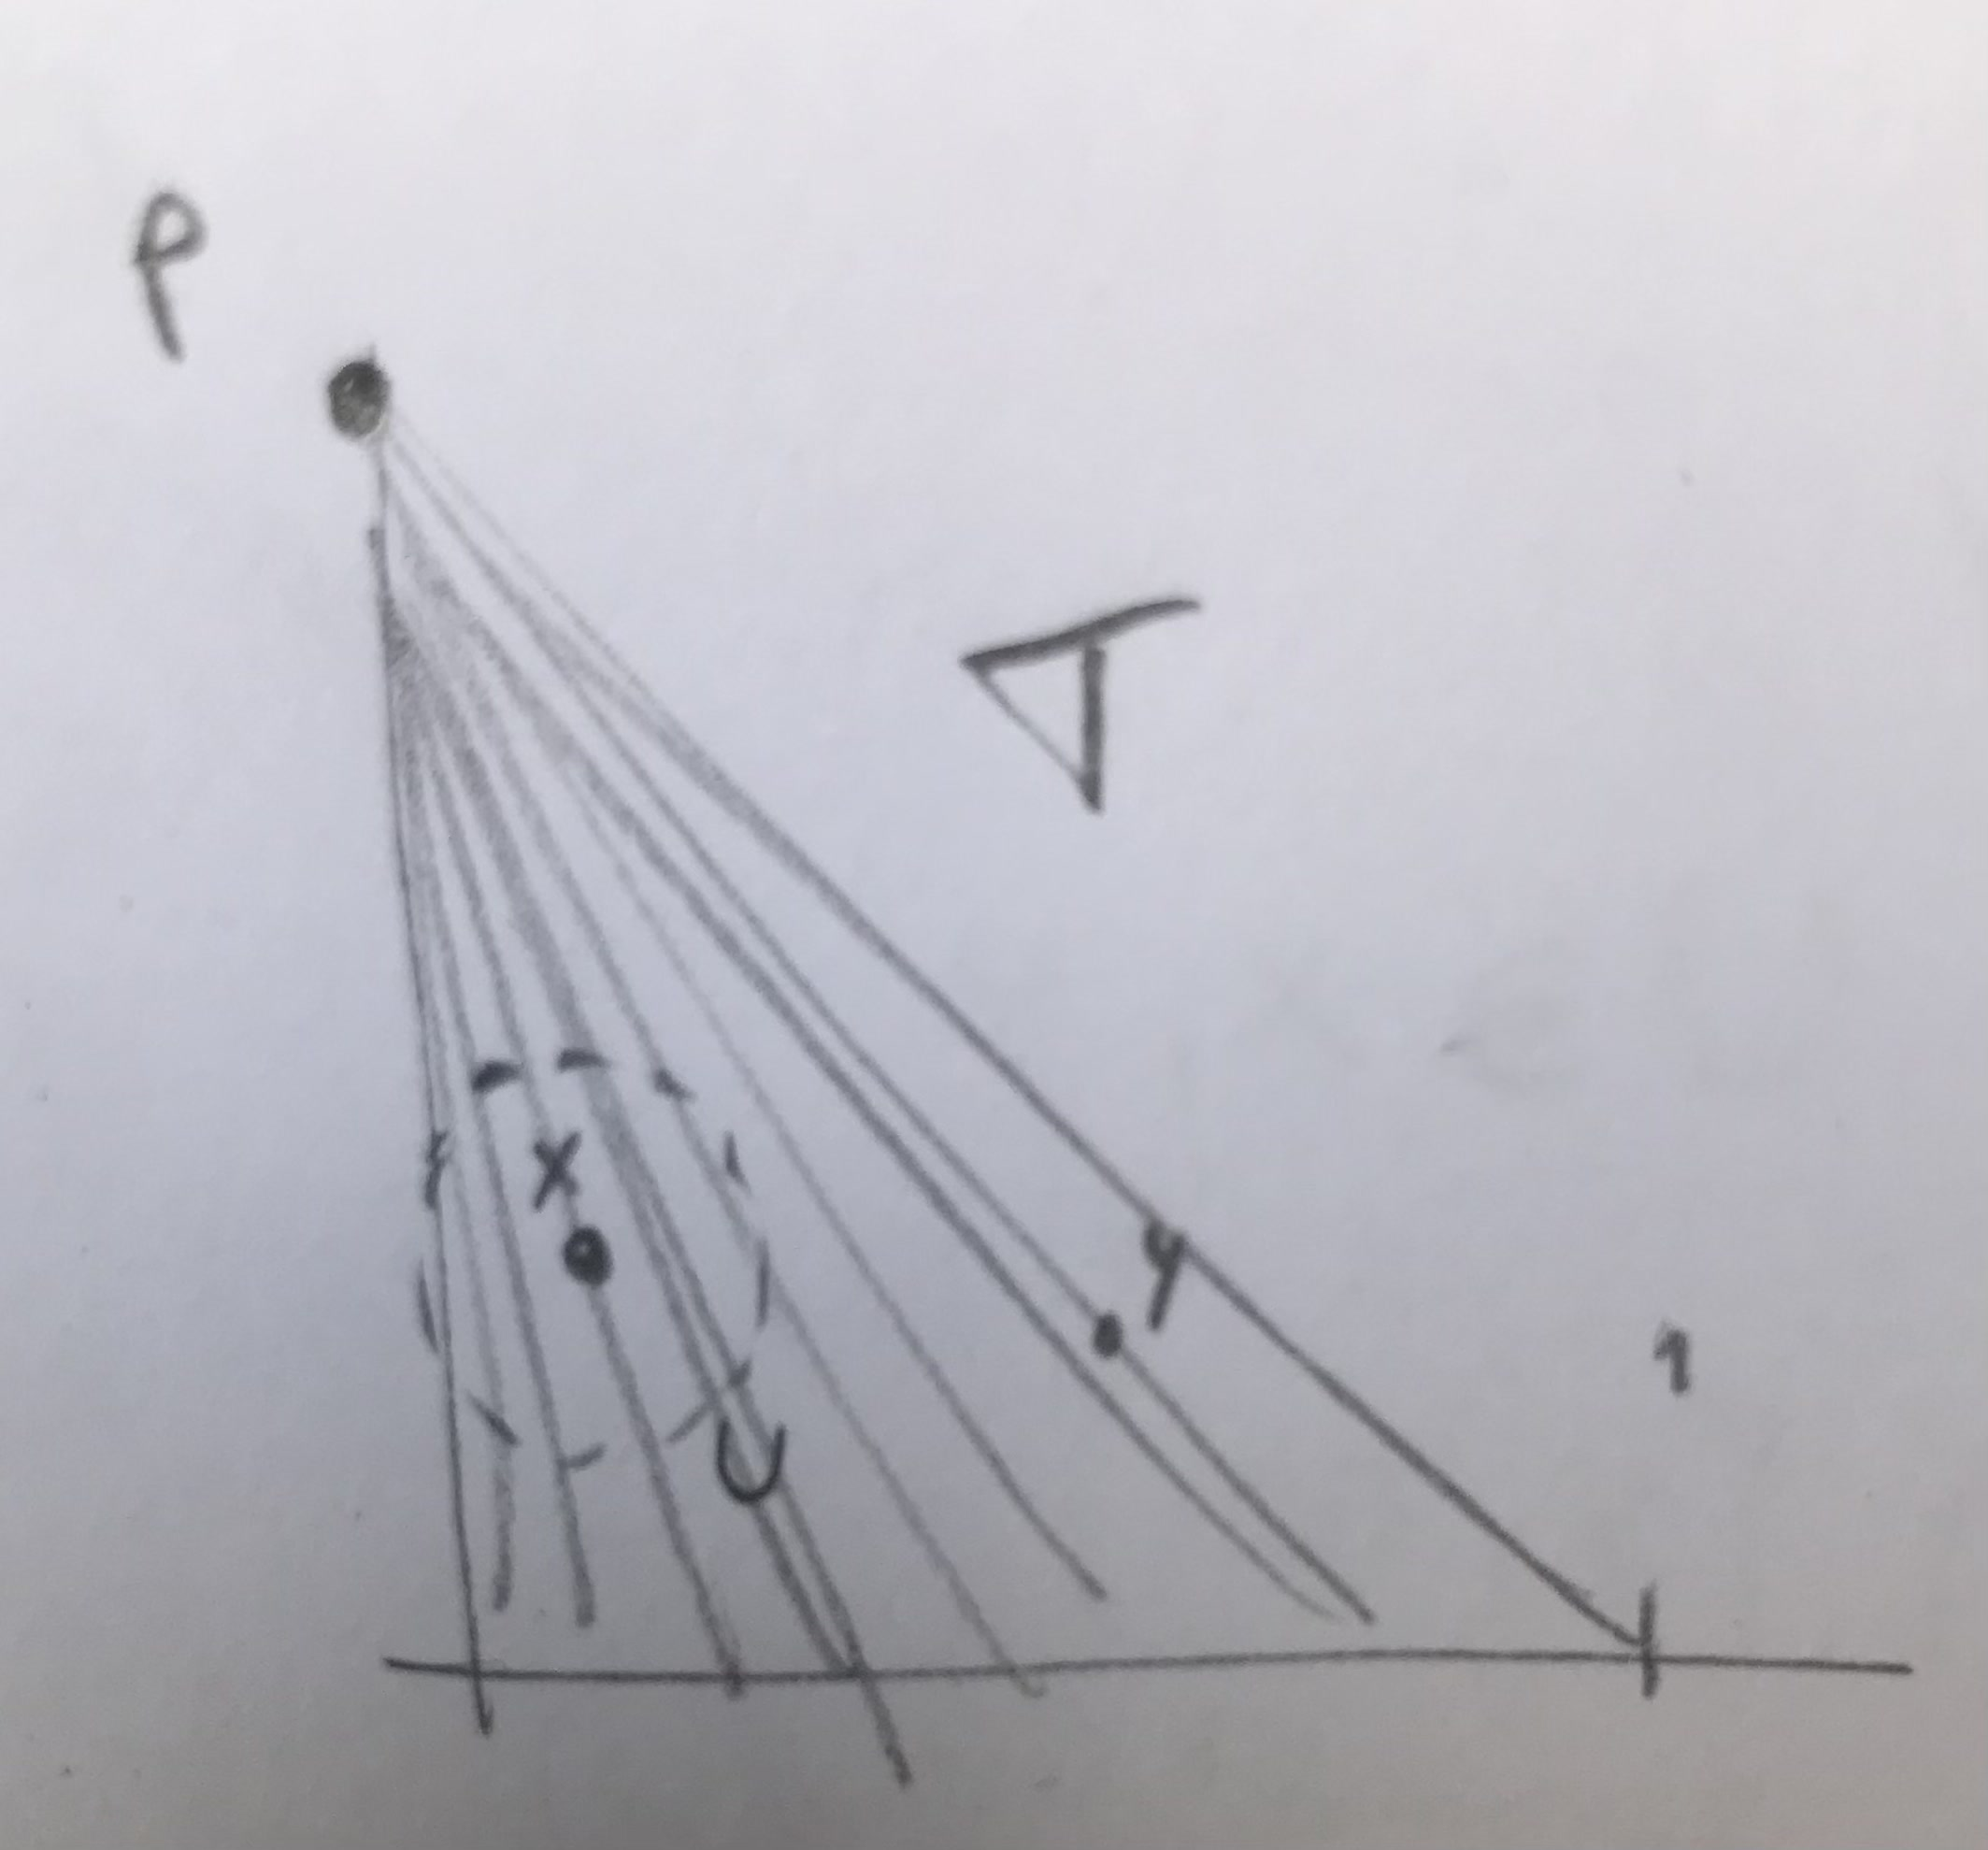
\includegraphics[scale=0.05]{Images/25-5-a.jpg}
    \end{figure}
    
    Now let's prove that it is only locally connected at $p$. The ball in $p$ is path connected, given $x\in T$, $x\neq p$, the ball $B(x,r)$ is formed by disjoint line segments, so we can separate the ball into two parts using a line that is not in $T$ for which its preimage is an irrational number.
    \item Let $T'$ be union of all line segments joining $1\times 0$ to the rational points of $[0,1]\times\{ 1 \}$, the union $T\cup T'$ is path connected but locally connected at none of its points.
    \begin{figure}[H]
      \centering
      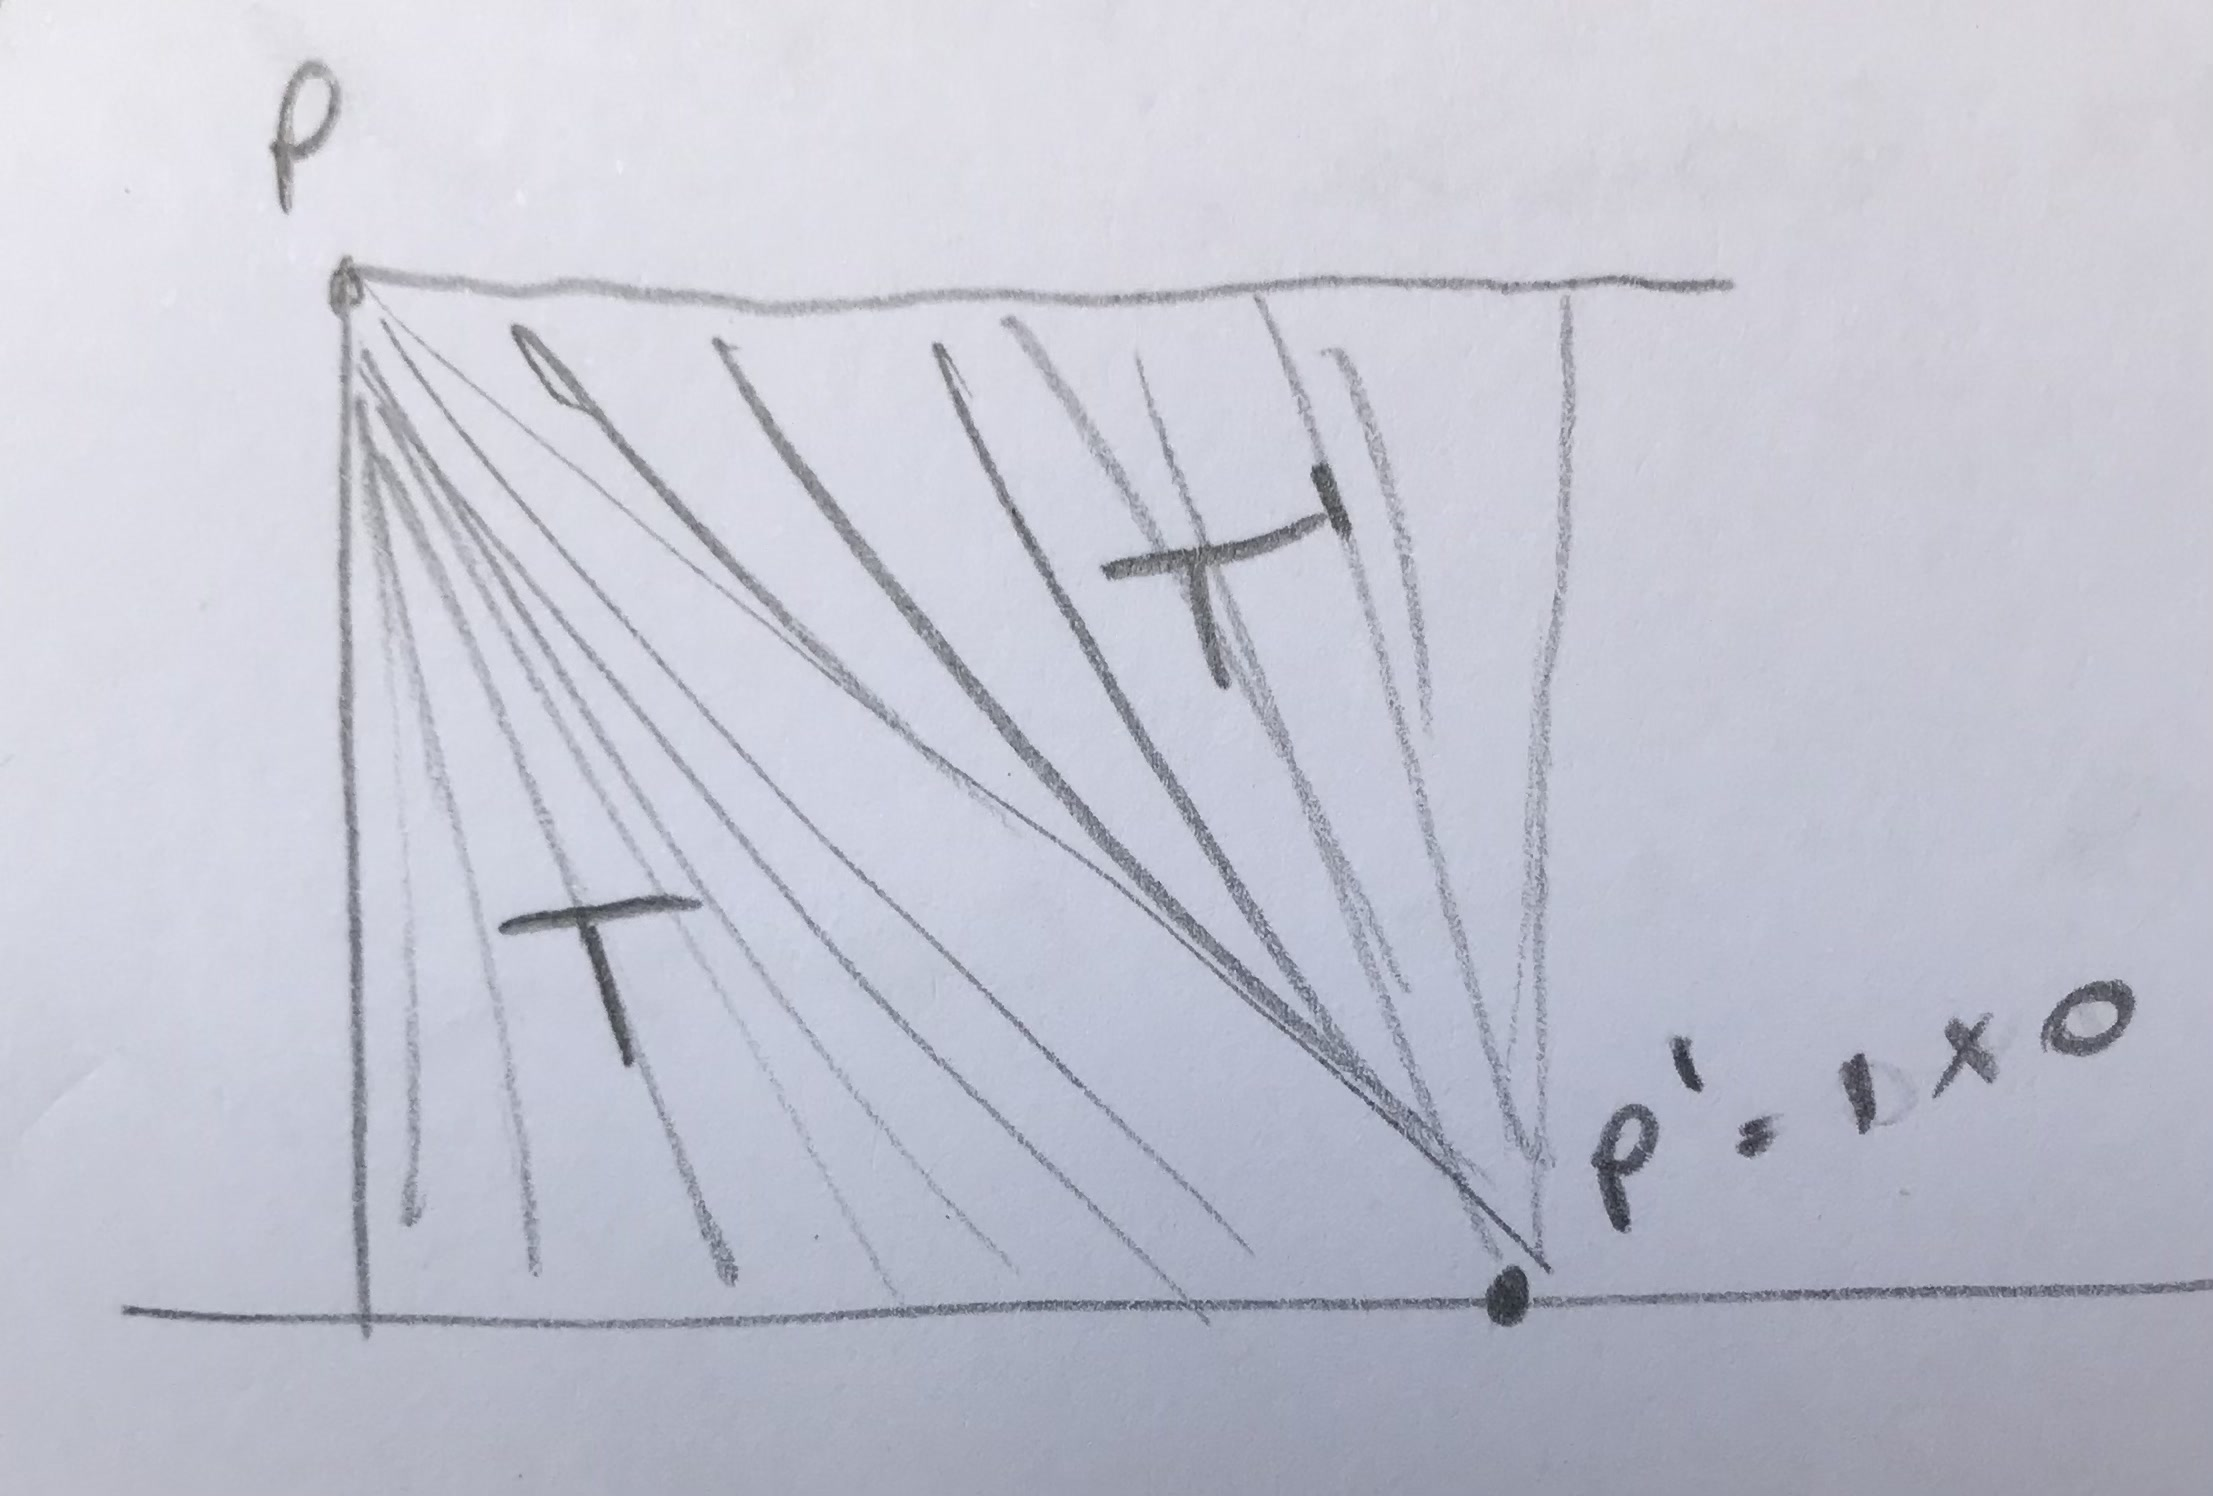
\includegraphics[scale=0.05]{Images/25-5-b.jpg}
    \end{figure}
  \end{enumerate}
\end{solution}

\section*{Section 26: Connectedness and Compactness}
\addcontentsline{toc}{section}{\protect\numberline{}Section 26: Connectedness and Compactness}

\begin{exerr}{1}\hfill
  \begin{enumerate}[label=(\alph*)]
    \item Let $\T$ and $\T'$ be two topologies on the set $\X$; suppose that $\T'\supset\T$. What does compactness of $\X$ under one of these topologies imply about compactness about the other?
    \item Show that if $\X$ is compact Hausdorff under both $\T$ and $\T'$, then either $\T$ and $\T'$ are equal or they are not comparable.
  \end{enumerate}
\end{exerr}
\begin{solution}\hfill
  \begin{enumerate}[label=(\alph*)]
    \item If $\X$ is compact in $\T'$ then it is compact in $\T$ because if $\{ A_{\alpha} \}_{\alpha}\subset\T$ is a convering of $\X$ then $\{ A_{\alpha} \}_{\alpha}\subset\T'$ and there exists a finite covering $\{ A_{\alpha_{i}} \}_{i=1}^m$, and $\{ A_{\alpha_{i}} \}_{i=1}^m\subset\T$. The other inclusion does not work, in $\R$, $\T_{\text{finite complement}}\subset\T_{\text{standard}}$. In the finite complement topology $(a,b)$ is compact but not in the standard
    \item Suppose $\T\subset\T'$, the identity function $f:(\X,\T)\to(\X,\T')$ is bijective and continuous and maps compact sets into compact sets. Given $U\subset\X$, $f(U)$ is open if and only if $U$ is open.
  \end{enumerate}
\end{solution}

\begin{exerr}{2}\hfill
  \begin{enumerate}[label=(\alph*)]
    \item Show that in the finite complement topology on $\R$, every subspace is compact.
    \item If $\R$ has the topology consisting of all sets $A$ such that $\R\backslash A$ is either countable or all of $\R$, is $[0,1]$ a compact subspace?
  \end{enumerate}
\end{exerr}
\begin{solution}
  \begin{enumerate}[label=(\alph*)]
    \item Let $\Y\subset\R$ with the finite complement topology, $\{ A_{\alpha} \}_{\alpha}$ a covering of $\Y$. Given that each $A_{\alpha}$ is open, it covers all but finite elements of $\Y$. Therefore, take one $A_{\alpha_{0}}$ and then finite $A_{\alpha_{i}}$ for $i=1,\dots,m$ such that those cover the ones $A_{\alpha}$ misses. The family $\{ A_{\alpha_{i}} \}_{i=0}^m$ is a finite covering of $\Y$.
    \item $[0,1]$ is not compact in the countable complement topology, let $A_{N} = \{ 1/n : n\geq N \}$. The sets $B_{N}=[0,1]\backslash A_{N}$, $\R\backslash B_{N} = A_{N}$ is countable, therefore $B_{N}\in\T$. $\bigcup B_{N}$ covers $[0,1]$ but there is no finite subcover.
  \end{enumerate}
\end{solution}

\begin{exerr}{3}
  Show that a finite union of compact subspaces of $\X$ is compact.
\end{exerr}
\begin{solution}
  Let $\X_{1},\X_{2},\dots,\X_{N}$ be compact subspaces of $\X$ and $\{ A_{\alpha} \}_{\alpha}$ a covering of $\bigcup_{i=1}^N\X_{i}$. Then $\{ A_{\alpha} \}$ is a cover of each $\X_{i}$, therefore there exists for each $i$ a finite subcover $\{ A_{\alpha_{j}}^i \}_{j=1}^{m_{i}}$, $\bigcup_{i=1}^N\bigcup_{j=1}^{m_{i}}A_{\alpha_{j}}^i$ is a finite cover of the union.
\end{solution}

\begin{exerr}{4}
  Show that every compact subspace of a metric space is bounded in that metric and is closed. Find a metric space in which not every closed bounded subspace is compact.
\end{exerr}
\begin{solution}
  Metric spaces are Hausdorff, therefore, $\X$ is Hausdorff and $\Y\subset\X$ is compact, then it is closed. Suppose that $\Y$ is not bounded, then for every $x\in\X$ and $r>0$ there exists $y\in\Y$ such that $y\notin B(x,r)$. The union of all such balls is a covering of $\X$, but there does not exist a finite covering of $\Y$. Absurd, then $\Y$ is bounded.

  Consider the space $(\R,\overline{d})$, $\overline{d}\not\sim d$, but $\T_{\overline{d}} = \T_{d}$, then they have the same compact sets, but with $\overline{d}$, $\R$ is bounded, but it is not compact.
\end{solution}

\begin{exerr}{5}
  Let $A$ and $B$ be disjoint compact subspaces of the Hausdorff space $\X$. Show that there exist disjoint open sets $U$ and $V$ containing $A$ and $B$, respectively.
\end{exerr}
\begin{solution}
  We know (Lemma 26.4) that for each $a\in A$, as $B$ is compact and $A\cap B=\varnothing$, there exist disjoint open sets $U_{\alpha}\ni a$ and $V_{\alpha}\supset B$. Clearly $\{ U_{a} \}_{a\in A}$ is a covering of $A$, and given that $A$ is compact, there exists a finite subcover $\{ U_{a_{i}} \}_{i=1}^m$. Defining $V = \bigcap_{i=1}^m V_{a_{i}}$ and $U = \bigcup_{i=1}^m U_{a_{i}}$ we have $U\cap V =\varnothing$, $U\supset A$, $V\supset V$ and $U,V$ open sets.
\end{solution}

\begin{exerr}{7}
  Show that if $\Y$ is compact, then the projection $\pi_{1}:\X\times\Y\to\X$ is a closed map.
\end{exerr}
\begin{solution}
  Define $B = \pi_{1}(A)$. Given $x_{0}\notin B$, $x_{0}\times\Y\cap A = \varnothing$. $(\X\times\Y)\backslash A$ is open and contains $x_{0}\times\Y$, then (tube lemma) it contains $W\times\Y$ with $W$ an open set in $\X$ that contains $x_{0}$.
  
  Doing this for each $x_{0}\notin B$ we obtain $B = \Big( \bigcup_{x\notin B}W_{x} \Big)^c$, therefore $B$ is closed.
\end{solution}

\begin{exerr}{8}
  Theorem. Let $f:\X\to\Y$ be compact Hausdorff. Then $f$ is continuous if and only if the graph of $f$,
  \begin{equation*}
      G_{f} = \{ x\times f(x) : x\in\X \},
  \end{equation*}
  is closed in $\X\times\Y$. [Hint: If $G_{f}$ is closed and $V$ is a neighourhood of $f(x_{0})$, then the intersection of $G_{f}$ and $\X\times(\Y\backslash V)$ is closed. Apply Exercise 7.]
\end{exerr}
\begin{solution}\hfill
  \begin{itemize}
    \item[($\Longrightarrow$)] $f$ is continuous, if $x\times y\in \X\times\Y$ is such that $x\times y\notin G_{f}$ then $y\neq f(x)$ and because $\Y$ is Hausdorff there exist open sets in $\Y$, $U,V$ such that $U\cap V=\varnothing$, $U\ni f(x)$ and $V\ni y$. Given that $f$ is continuous, $f^{-1}(U)$ is open and $x\in f^{-1}(U)$.
    
    $f^{-1}(U)\times V$ is a neighbourhood of $x\times y$ and $(f^{-1}(U)\times V)\cap G_{f} = \varnothing$, because if it wasn't then there would exist $x_{0}\in f^{-1}(U)$ such that $f(x_{0})\in V$, but $U\cap V = \varnothing$.
    \item Let $x_{0}\in\X$, $V$ neighbourhood of $f(x_{0})$, $\X\times V$ is open, $\Y\backslash V$ is closed and $G_{f}\cap\big( \X\times(\Y\backslash V) \big)$ is closed. Using exercise 7, as $\Y$ is compact, $\pi_{1}:\X\times\Y\to\X$ is closed, then $\pi_{1}\big(G_{f}\cap\big( \X\times(\Y\backslash V) \big)\big)$ is closed.
    \begin{equation*}
        \pi_{1}\big(G_{f}\cap\big( \X\times(\Y\backslash V) \big)\big) = (f^{-1}(V))^c,
    \end{equation*}
    then $f^{-1}(V)$ is open and $f$ is continuous.
  \end{itemize}
\end{solution}

\section*{Section 27: Compact Subspaces of the Real Line}
\addcontentsline{toc}{section}{\protect\numberline{}Section 27: Compact Subspaces of the Real Line}

\begin{exerr}{1}
  Prove that if $\X$ is an ordered set in which every closed interval is compact, then $\X$ has the least upper bound property.
\end{exerr}
\begin{solution}
  Let $A\subset\X$ be a set bounded by some $x\in\X$, that is, for every $a\in A$, $a\leq x$. If $x\in A$, then $x$ is the least upper bound and there is nothing to prove. If $x\notin A$ but $x = a+1$ for some $a\in A$, then $a$ is the least upper bound. If none of these situations occur, define the set $B$ formed by all the upper bounds of $A$ and consider the family $\C$ of intervals $[a,b]$ with $a\in A$ and $b\in B$. $\C$ has the finite intersection property, then there exists $c\in\bigcap_{[a,b]\in\C}[a,b]$, $c$ is the least upper bound.
\end{solution}

\begin{exerr}{2}
  Let $\X$ be a metric space with metric $d$; let $A\subset\X$ be nonempty.
  \begin{enumerate}[label=(\alph*)]
    \item Show that $d(x,A)=0$ if and only if $x\in \overline{A}$.
    \item Show that if $A$ is compact, $d(x,A) = d(x,a)$ for some $a\in A$.
    \item Define the $\varepsilon$-neighbourhood of $A$ in $\X$ to be the set
    \begin{equation*}
        U(A,\varepsilon) = \{ x : d(x,A)<\varepsilon \}.
    \end{equation*}

    Show that $U(A,\varepsilon)$ equals the union of the open balls $B_{d}(a,\varepsilon)$ for $a\in A$.
    \item Assume that $A$ is compact; let $U$ be an open set containing $A$. Show that some $\varepsilon$-neighbourhood of $A$ is contained in $U$.
    \item Show the result in (d) need not hold if $A$ is closed but not compact.
  \end{enumerate}
\end{exerr}
\begin{solution}
  \begin{enumerate}[label=(\alph*)]

    \item\hfill
    
    \begin{itemize}
      \item[($\Longleftarrow$)] If $x\in \overline{A}$ then for every neighbourhood $U$ of $x$, $(U\cap A)\backslash\{ x \}=\varnothing$. $\{ B(x,1/n) \}$ is a family of neighbourhoods of $x$ and for every $n\in\N$ there exists $y\in(B(x,1/n)\cap A)\backslash\{ x \}$, that is, $d(y,x)<n$, therefore, $d(x,A)=0$.
      \item[($\Longrightarrow$)] If $d(x,A)=0$ then for every $n$ there exists $y\in A$ such that $d(x,y)<1/n$, then $y\in B(x,1/n)$ and with this $(B(x,1/n)\cap A)\backslash\{ x \}\neq \varnothing$ for every $n$, therefore, $x\in \overline{A}$.
    \end{itemize}
    \item Let $d:\X\times\X\to\R$, be the distance function $d(x,A)$. We know that $d$ is continuous and because $A$ is compact, it reaches its minimum value at some point $a\in A$, then $d(x,a) = d(x,A)$.
    \item Let's prove the double inclusion.
    \begin{itemize}
      \item[($\supset$)] Let $x\in\bigcup_{a\in A}B_{d}(a,\varepsilon)$, then $x\in B_{d}(a,\varepsilon)$ for some $a\in A$ and $d(x,a)<\varepsilon$, then $d(x,A)<\varepsilon$ and $x\in U(A,\varepsilon)$.
      \item[($\subset$)] Let $x\in U(A,\varepsilon)$, $d(x,A)<\varepsilon$, this happens if and only if $d(x,a)<\varepsilon$ for some $a\in A$, then $x\in B_{d}(a,\varepsilon)$.
    \end{itemize}
    \item Let $\big\{ B\big(a,d(a,\X\backslash U)\big) \big\}$ be a covering of $A$. Because $A$ is compact, there exists a finite subcovering $\big\{ B\big(a_{i},d(a_{i},\X\backslash U)\big) \big\}$, let $\varepsilon = \min_{1\leq i\leq N}d(a_{i},\X\backslash U)$, then $U(A,\varepsilon) = \bigcup_{a\in A}B(a,\varepsilon)\subset U$.
    \item In $\R\times\R$ the set $\{ x\times \frac{1}{x} : x>0 \}$ is closed but not compact.
  \end{enumerate}
\end{solution}

\begin{exerr}{3}
  Recall that $\R_{K}$ denotes $\R$ in the $K$-topology.
  \begin{enumerate}[label=(\alph*)]
    \item Show that $[0,1]$ is not compact as a subspace of $\R_{K}$.
    \item Show that $\R_{K}$ is connected. [Hint: $(-\infty,0)$ and $(0,\infty)$ inherit their usual topologies as subspaces of $\R_{K}$.]
    \item Show that $\R_{K}$ is not path connected.
  \end{enumerate}
\end{exerr}
\begin{solution}\hfill
  \begin{enumerate}[label=(\alph*)]
    \item $(-1,2)\backslash K \cup\{ (1/n,1) \}_{n=1}^\infty$ is a cover of $[0,1]$, but there does not exist a finite subcovering.
    \item Suppose that $\R_{K}$ is not connected, then there exist open sets $U,V$ such that $\R_{K} = U\cup V$. The sets $(-\infty, 0)$ and $(0,\infty)$ are connected, so let suppose $(0,\infty)\subset V$ and $(-\infty,0)\subset U$, if $0\in U$ then $(-\infty,0]$ is open and closed at the same time, absurd, then $\R_{K}$ is connected.
    \item Suppose there exists $f:[a,b]\to[0,1]$ such that $f(a) = 0$, $f(b) = 1$. Given that the usual topology is contained in the $K$-topology then $f$ is surjective, then $f([a,b]) = [0,1]$, then $[0,1]$ should be compact in $\R_{K}$, which does not happen. Therefore, $\R_{K}$ is not path connected.
  \end{enumerate}
\end{solution}

\begin{exerr}{4}
  Show that a connected metric space having more than one point in uncountable.
\end{exerr}
\begin{solution}
Given that the distance function is continuous, it maps connected sets onto connected sets, given $x\in\X$, the function $d_{x}:\X\to\R$ given by $d_{x}(y) = d(x,y)$ is continuous. Since $\X$ is connected $d_{x}(\X)$ is connected and contains $0$ because $d_{x}(x) = 0$. Thus, if $y\in\X$ and $y\neq x$, then $d_{x}(\X)$ contains the set $[0,\delta]$, where $\delta = d_{x}(y)>0$. Then $\X$ must be uncountable.
\end{solution}

\section*{Section 28: Limit Point Compactness}
\addcontentsline{toc}{section}{\protect\numberline{}Section 28: Limit Point Compactness}

\begin{exerr}{1}
  Give $[0,1]^\omega$ the uniform topology. Find an infinite subset of this space that has no limit point.
\end{exerr}
\begin{solution}
  Each point of the point $x_{n} = (0,\dots,1,0,\dots)$ with $1$ in the $n$-th component is isolated in the sequence, because $\overline{\rho}(x_{n},x_{m}) = 1$ for all $n\neq m$, therefore it cannot have a limit point.
\end{solution}

\begin{exerr}{2}
  Show that $[0,1]$ is not limit point compact as a subspace of $\R_{\ell}$.
\end{exerr}
\begin{solution}
  The set $A = \{ 1-\frac{1}{n} : n\in\N \}$ has no limit points in $\R_{\ell}$, there exists a neighbourhood $[1,2)\cap [0,1]$ that do not contain points of $A$, and if $x\in[0,1]$, $x\neq1$ then there exists $N\in\N$ such that
  \begin{equation*}
      \frac{1}{N-1}\leq x < 1 - \frac{1}{N},
  \end{equation*}
  is a neighbourhood of $x$ that does not intersect $A$.
\end{solution}

\begin{exerr}{3}
  Let $\X$ be limit point compact.
  \begin{enumerate}[label=(\alph*)]
    \item If $f:\X\to\Y$ is continuous, does it follow that $f(\X)$ is limit point compact?
    \item If $A$ is a closed subset of $\X$, does it follow that $A$ is limit point compact?
  \end{enumerate}
\end{exerr}
\begin{solution}\hfill
  \begin{enumerate}[label=(\alph*)]
    \item No, we know that $\X = \Z\times\{ a,b \} $ is limit point compact and the projection $\pi_{1}$ is continuous, but $\pi_{1}(\X) = \Z$ is not limit point compact.
    \item Yes, if $B\subset A$ is an infinite set has limit points in $\X$ then they must be in $A$ because it is closed.
  \end{enumerate}
\end{solution}

\begin{exerr}{4}
  A space $\X$ is said to be countably compact if every countable open covering of $\X$ contains a finite subcollection that covers $\X$. Show that for a $T_{1}$ space $\X$, countable compactness is equivalent to limit point compactness. [Hint: If no finite subcollection of $U_{n}$ covers $\X$, choose $x\notin U_{1}\cup\cdots U_{n}$, for each $n$.]
\end{exerr}
\begin{solution}\hfill
  \begin{itemize}
    \item[($\Longrightarrow$)] Let $\Y\subset\X$ be an infinite set and $Z\subset\Y$ countable, $Z =\{ x_{n} \}_{n}$. Suppose that no point in $Z$ is limit point, then for every $n_{0}$ there exists a neighbourhood $U_{n_{0}}$ of $x_{n_{0}}$ such that $U_{n_{0}}\cap Z = \{ x_{n_{0}} \}$. Because $Z$ is closed, $\{ U_{n} \}\cup(\X\backslash Z)$ is open and countable, but it does not contain a finite subcovering. Thus, $Z$ cannot be closed and this means that there exists a limit point of $Z$ which is not in $Z$.
    \item[($\Longleftarrow$)] Let $\{ U_{n} \}_{n}$ be a countable covering of $\X$, define $V_{n} = \bigcup_{i=1}^n U_{i}$. If there is no finite subcover of $\{ U_{n} \}$ then for each $n$ there exists $x_{n}\notin V_{n}$. Let $\{ x_{n} \}$ the sequence formed this way, this sequence has a limit point $a$, $a\in V_{n_{0}}$ for some $n_{0}$ but $V_{n_{0}}$ contains only finite points in the sequence. Given that $a$ is a limit point in a $T_{1}$ space, every neighbourhood of $a$ has infinite points, therefore, there exists $N$ such that $V_{N}$ covers $\X$, thus, $\X$ is countably compact.
  \end{itemize}
\end{solution}

\begin{exerr}{5}
  Show that $\X$ is countably compact if and only if every nested sequence $C_{1}\supset C_{2}\supset\cdots$ of closed nonempty sets of $\X$ has a nonempty intersection.
\end{exerr}
\begin{solution}\hfill
  \begin{itemize}
    \item[($\Longrightarrow$)] Let $\A = \{ \X\backslash C_{i} : i\in\N \}$, $\A$ covers $\X$ if and only if $\bigcap C_{i} = \varnothing$. Therefore, $\A$ does not contain any finite subcover, because if it did, then it would be $\bigcap_{i=1}^m C_{i}= \varnothing$ and that cannot happen because $C_{1}\supset C_{2}\supset\cdots$. Because $\A$ does not cover $\X$ there exists $x\in\X$ such that $x\notin \A$, then $x\in\bigcap_{i=1}^\infty C_{i}$.
    \item[($\Longleftarrow$)] Let $\{ A_{i} \}_{i\in\N}$ be a covering of $\X$. Define the closed sets $B_{n} = \X\backslash \big( \bigcup_{i\leq n}A_{i} \big)$, which satisfy $B_{1}\supset B_{2}\supset\cdots$, then $\bigcap B_{i} \neq \varnothing$,
    \begin{equation*}
        \Big( \bigcap B_n \Big)^c = \bigcup A_{i} = \X,
    \end{equation*}
    then there exists $N\in\N$ such that $B_{N}\neq \varnothing$, thus, $\bigcup^N_{i=1} A_{i} = \X$
  \end{itemize}
\end{solution}

\section*{Section 30: The Countability Axioms}
\addcontentsline{toc}{section}{\protect\numberline{}Section 30: The Countability Axioms}

\begin{exerr}{1}\hfill
  \begin{enumerate}[label=(\alph*)]
    \item A $G_{\delta}$ set in a space $\X$ is a set $A$ that equals a countable intersection of open sets on $\X$. Show that in a first-countable $T_{1}$ space, every one-point set is a $G_{\delta}$ set.
    \item There is a familiar space in which every one-point set is a $G_{\delta}$ set, which nevertheless does not satisfy the first countability axiom. What is it?
  \end{enumerate}
\end{exerr}
\begin{solution}\hfill
  \begin{enumerate}[label=(\alph*)]
    \item Let $x\in\X$ and let $\B = \{ B_{n} \}_{n\in\N}$ be a countable base for $x$, let's see that $x = \bigcap_{n}B_{n}$.
    
    Let $y\in\cap_{n}B_{n}$, suppose by contradiction that $y\neq x$. Given that $\X$ is $T_{1}$ we know that there exist neighbourhoods $U,V$ of $x$ and $y$ respectively such that $y\notin U$ and $x\notin V$. Because $\X$ is 1° countable then there exists $n_{0}$ such that $B_{n_{0}}\subset U$ and $y\in B_{n_{0}}$, which is a contradiction. Then $x = \bigcap_{n}B_{n}$.
    \item $\R^\omega$ with $\T_{\text{box}}$ is not 1° countable, but given $x\in\R^\omega$ let $U_{n}^i = (x_{i}-1/n, x_{i}+1/n)$, $\{ U_{n}^i \}_{n}$ is a local basis of each $x_{i}$ such that $\bigcap_{n}U_{n}^i = \{ x_{i} \}$, therefore, $\bigcap_{n}\big( \prod_{i}U_{n}^i \big) = \{ x \}$.
   \end{enumerate}
\end{solution}

\begin{exerr}{4}
  Show that every compact metrizable space $\X$ has a countable basis. [Hint: Let $\A_{n}$ be a finite covering of $\X$ by $1/n$ balls.]
\end{exerr}
\begin{solution}
  Let $\{ B(x,1/n) \}_{x\in\X}$ be a covering of $\X$, because it is compact, there exists a finite subcover $\{ B(x_{i},1/n) \}_{i=1}^{m(n)}$. Consider $\B = \bigcup_{n\in\N}\{ B(x_{i},1/n) \}_{i=1}^{m(n)}$, $\B$ is a basis:
  \begin{enumerate}
    \item If $x\in\X$ then $x\in B(x_{i},1/n)$ for some $i$ and $n$, because $\{ B(x_{i},1/n) \}$ was a cover of $\X$.
    \item If $x\in B(x_{i},1/n_{i})\cap B(x_{j},1/n_{j})$ then there exist $r_{i}$, $r_{j}$ and $y$ such that $B(y,r_{i})\subset B(x_{i},1/n_{i})$ and $B(y,r_{j})\subset B(x_{j},1/n_{j})$. Taking $r = \min(r_{1},r_{2})$ we have that there exists $B(x_{n_{0}},1/n_{0}) \subset B(y,r)$ that contains $x$.
  \end{enumerate}
\end{solution}

\begin{exerr}{5}\hfill
  \begin{enumerate}[label=(\alph*)]
    \item Show that every metrizable space with a countable dense subset has a countable basis.
    \item Show that every metrizable Lindelöf space has a countable basis.
  \end{enumerate}
\end{exerr}
\begin{solution}\hfill
  \begin{enumerate}[label=(\alph*)]
    \item If $D\subset\X$ is a countable dense set then $\B = \bigcup_{n\in\N}\{ B(d,1/n) \}_{d\in D}$, is a countable basis of $\X$.
    \item Given $n\in\N$, $\{ B(x,1/n) \}_{x\in\X}$ is a covering of $\X$, and because $\X$ is Lindelöf, there exists a countable subcovering $\{ B(x_{i},1/n) \}_{i\in\N}$. The set $\B = \bigcup_{n\in\N}\{ B(x_{i},1/n) \}_{i\in\N}$ is a countable basis of $\X$.
  \end{enumerate}
\end{solution}

\begin{exerr}{6}
  Show that $\R_{\ell}$ and $I_{0}^2$ are not metrizable.
\end{exerr}
\begin{solution}
  We know that Lindelöf + Metrizable $\implies$ 2° countable. As $\R_{\ell}$ is not 2° countable and is Lindelöf, then it cannot be metrizable. Also, Compact + Metrizable $\implies$ Separable, $I_{0}^2$ is compact, because us it is a linear continuum, then it also cannot be metrizable, because it is not separable.
\end{solution}

\begin{exerr}{8}
  Which of our four countability axioms does $\R^\omega$ in the uniform topology satisfy?
\end{exerr}
\begin{solution}
  We've seen in the book that $\R^\omega$ with the uniform topology is 1° countable, it is not 2° countable (done in the book), It is also not Lindelöf nor separable because of what we've proven in Exercise 5.
\end{solution}

\begin{exerr}{9}
  Let $A$ be a closed subspace of $\X$. Show that if $\X$ is Lindelöf, then $A$ is Lindelöf. Show by example that if $\X$ has a countable dense subset, $A$ need not have a countable dense subset.
\end{exerr}
\begin{solution}
  Let $\{ A_{\alpha} \}_{\alpha}$ be an open cover of $A$. $\{ A_{\alpha} \}_{\alpha}\cup\{ \X\backslash A \}$ is a covering of $\X$, and because it is Lindelöf then there exists a countable subcover $\{ A_{\alpha_{i}} \}_{i\in\N}\cup\{ \X\backslash A \}$, the family $\{ A_{\alpha_{i}} \}_{i\in\N}$ is a countable cover of $A$.

  \textbf{Example:} The Sorgenfray plane, $A = L = \{ x\times(-x) : x\in\R_{\ell} \}$
\end{solution}

\begin{exerr}{11}
  Let $f:\X\to\Y$ be continuous. Show that if $\X$ is Lindelöf, or if $\X$ has a countable dense subset, then $f(\X)$ satisfies the same condition.
\end{exerr}
\begin{solution}\hfill
  \begin{itemize}
    \item $\X$ Lindelöf. Let $\{ B_{\alpha} \}_{\alpha}$ be a covering of $f(\X)$, the set $A_{\alpha} = f^{-1}(B_{\alpha})$ is open in $\X$ and covers it. Then there exists a countable subcover $\{ f^{-1}(B_{\alpha_{i}}) \}_{i\in\N}$, the family $\{ B_{\alpha_{i}} \}_{i\in\N}$ is a countable subcover of $f(\X)$.
    \item $\X$ separable. Let $D\subset\X$ be the countable dense set in $\X$, then $\overline{f(D)} = f(\overline{D}) = = f(\X)$.
  \end{itemize}
\end{solution}

\begin{exerr}{14}
  Show that if $\X$ is Lindelöf and $\Y$ is compact, then $\X\times\Y$ is Lindelöf.
\end{exerr}
\begin{solution}
  We will take a covering formed by elements of the basis $\{ U_{\alpha}\times V_{\alpha} \}_{\alpha}$ of $\X\times\Y$. Given $x_{0}\in\X$, $x_{0}\times\Y$ is compact and there exists $\{ U_{\alpha_{i}}\times V_{\alpha_{i}} \}_{i=1}^m$, a finite subcover of $x_{0}\times\Y$. Let $U_{x_{0}} = \bigcap_{i=1}^m U_{\alpha_{i}}$. The family $\{ U_{x} \}_{x\in\X}$ is a covering of $\X$ and there exists a countable subcover $\{ U_{x_{n}}^i \}_{i\in\N}$. Consider the countable family $\{ U_{x_{n}}^i\times V_{x_{n}}^i \}_{i\in\N}$. Let $x\times y\in\X\times\Y$, $x\in U_{x_n}$ for some $n$, then $x\times y\in U_{x_{n}}^i\times V_{x_{n}}^i$ for some $i$, and so the family in consideration is a countable subcover of $\X\times\Y$.
\end{solution}

\section*{Section 31: The Separation Axioms}
\addcontentsline{toc}{section}{\protect\numberline{}Section 31: The Separation Axioms}

\begin{exerr}{1}
  Show that if $\X$ is regular, every pair of points of $\X$ have neighbourhoods whose closures are disjoint.
\end{exerr}
\begin{solution}
  Let $x,y\in\X$ be distinct points, given that singletons are closed sets, there exist $U,V$ neighbourhoods of $x$ and $y$ such that $U\cap V = \varnothing$. Because $\X$ is regular, there exist $U'$ and $V'$ such that $x\in U'\subset \overline{U'}\subset U$ and $y\in V'\subset \overline{V'}\subset V$, thus $\overline{U'}\cap\overline{V'} = \varnothing$.
\end{solution}

\begin{exerr}{2}
  Show that if $\X$ is normal, every pair of disjoint closed sets have neighbourhoods whose closures are disjoint.
\end{exerr}
\begin{solution}
  Let $A,B$ be closed disjoint subsets of $\X$. There exist open sets $U,V$ such that $A\subset U$, $B\subset V$ and $U\cap V = \varnothing$. Because $\X$ is normal we know that there exist $U', V'$ such that $A\subset U'\subset\overline{U'}\subset U$ y $B\subset V'\subset\overline{V'}\subset V$, then $U'$ and $V'$ are neighbourhoods of $A$ and $B$ such that $\overline{U'}\cap\overline{V'} = \varnothing$.
\end{solution}

\begin{exerr}{3}
  Show that every order topology is regular.
\end{exerr}
\begin{solution}\hfill
  \begin{itemize}
    \item $\{ x \}   = \big( (-\infty,x)\cup(x,\infty) \big)^c$.
    \item Let $x\in\X$, $A\subset \X$ closed sch that $x\notin A = \overline{A}$. Then there exists $(a,b)\ni x$ open set such that $(a,b)\cap A = \varnothing$. The set $V = (-\infty,a)\cup(b,\infty)$ is a neighbourhood of $A$ and $(a,b)\cap V = \varnothing$.
  \end{itemize}
\end{solution}

\begin{exerr}{4}
  Let $(\X,\T)$ and $(\X,\T')$ be two topological spaces with the same set such that $T\subset\T'$. If one of the spaces is Hausdorff (or regular, or normal), what does that imply about the other?
\end{exerr}
\begin{solution}
  If $(\X,\T)$ is Hausdorff then $(\X,\T')$ is Hausdorff, given $x,y\in\X$, $x\neq y$ there exist $U,V$ neighbourhoods of $x$ and $y$ such that $U\cap V = \varnothing$ and $U, V\in\T'$, so $(\X,\T')$ is Hausdorff. The other implication is not necessarily valid, in $\R$, $\T = \{ \varnothing,\R \}$ is contained in $\T' = \Par(\R)$, $\T'$ is Hausdorff but $\T$ is not.

  For normal and regular sets none of the implications are valid. The standard topology is regular and normal but the $K$-topology is neither regular nor normal. For the other direction take the $K$-topology, and $\T' = \Par(\R)$.
\end{solution}

\begin{exerr}{5}
  Let $f,g:\X\to\Y$ be continuous; assume that $\Y$ is Hausdorff. Show that $\{ x : f(x) = g(x) \}$ is closed in $\X$.
\end{exerr}
\begin{solution}
  Let $A = \{ x : f(x) = g(x) \}$, if $x\notin A$ then $f(x) \neq g(x)$ and because $\Y$ is Hausdorff there exist $U,V\subset\Y$ neighbourhoods of $f(x)$ and $g(x)$ such that $U\cap V = \varnothing$. The set $B = f^{-1}(U)\cap g^{-1}(V)$, is a neighbourhood of $x$ and $B\subset A^c$, then $A^c$ is open and $A$ is closed.
\end{solution}

\begin{exerr}{6}
  Let $p:\X\to\Y$ be a closed continuous surjective map. Show that if $\X$ is normal, then so is $\Y$. [Hint: If $U$ is an open set containing $p^{-1}(y)$, show there is a neighbourhood $W$ of $y$ such that $p^{-1}(W)\subset U$.]
\end{exerr}
\begin{solution}
  Singletons are closed because for every $x\in\X$, $\{ x \}$ is closed and given that $p$ is a closed surjective function, we have that $p(\{ x \}) = \{ y \}$ is closed.

  Let $B\subset\Y$ be a closed set and $V$ a neighbourhood of $B$. We want to prove that there exists an open set $Z$ such that $B\subset Z\subset \overline{Z}\subset V$. The sets $A = p^{-1}(B)$ and $U = p^{-1}(U)$ are closed and open respectively because $p$ is continuous. Given that $\X$ is normal, there exists an open set $W$ such that $A\subset W\subset \overline{W}\subset U$, then $\X\backslash W$ is closed and using that $p$ is surjective yields $P(W)\subset \Y\backslash p(\X\backslash W)$. Denoting $p(W)$ by $Z$ we have
  \begin{align*}
    B &= p(A)\subset Z\subset\Y\backslash p(\X\backslash W)\subset p(V),\\
    \overline{Z} &= \overline{p(W)} = p(\overline{W})\subset p(U) = V.
  \end{align*}

  Therefore, $\Y$ is normal.
\end{solution}

\section*{Section 32: Normal Spaces}
\addcontentsline{toc}{section}{\protect\numberline{}Section 32: Normal Spaces}

\begin{exerr}{1}
  Show that a closed subspace of a normal space is normal.
\end{exerr}
\begin{solution}
  Let $\X$ be a normal space, $\Y\subset\X$ a closed subspace. Let $A,B\subset\Y$ be closed sets, then $A = \widetilde{A}\cap\Y$ and $B = \widetilde{B}\cap\Y$ with $\widetilde{A},\widetilde{B}$ closed sets in $\X$. Given that $\X$ is normal, there exist disjoint neighbourhoods $U, V$ of $\widetilde{A}$ and $\widetilde{B}$, then $(U\cap\Y)\cap(V\cap\Y) = \varnothing$, $U\cap Y\supset A$ and $V\cap\Y\supset B$.
\end{solution}

\begin{exerr}{4}
  Show that every regular Lindelöf space is normal.
\end{exerr}
\begin{solution}
  It's very similar to the theorem, Regular and 2° countable imply normal, so we just need to know that it has a countable basis, for this consider a cover $a\in B_{n}\subset U_{n}$ and use the Lindelöf condition.
\end{solution}

\begin{exerr}{5}
  Is $\R^\omega$ normal in the product topology? In the uniform topology?
\end{exerr}
\begin{solution}
  $\R^\omega$ with both the product and uniform topology are metrizable, then they are normal.
\end{solution}


\section*{Section 33: The Urysohn Lemma}
\addcontentsline{toc}{section}{\protect\numberline{}Section 33: The Urysohn Lemma}

\begin{exerr}{1}
  Examine the proof of the Urysohn lemma, and show that for given $r$,
  \begin{equation*}
      f^{-1}(r) = \bigcap_{p>r}U_{p}\backslash\Big( \bigcup_{q<r} U_{q} \Big),
  \end{equation*}
  for $p,q$ rationals.
\end{exerr}
\begin{solution}
  We will prove it by double inclusion.
  \begin{itemize}
    \item[$\subset$:] Let $x\in f^{-1}(r)$, then $r = \inf\Q(x) = \inf\{ p : x\in U_{p} \}$, if $t\in \Q$ is such that $r<t$ then there exists $p<t$, $p\in\Q(x)$ such that $r<p<t$, then $x\in U_{p}$. Doing this for every $t>r$ we have $x\in\bigcap_{p>r}U_{p}$.
    
    If $q\in\Q$ is such that $r>q$, then $x\notin U_{q}$ because $r$ is the infimum, then $x\notin \bigcup_{q<r}U_{q}$.
    
    So $f^{-1}(r)\subset\bigcap_{p>r}U_{p}\backslash\Big( \bigcup_{q<r} U_{q} \Big)$.
    \item[$\supset:$] If $x\in\bigcap_{p>r}U_{p}\backslash \Big( \bigcup_{q<r} U_{q} \Big)$, then
    \begin{itemize}
      \item $x\in U_{p}\subset \overline{U}_{p}$ for every $p>r$, then $f(x) \leq r$,
      \item $x\notin U_{q}$ for every $q<r$, then $f(x) \geq r$.
    \end{itemize}
    Then $f(x) = r$ and $x\in f^{-1}(r)$.
  \end{itemize}
\end{solution}

\begin{exerr}{3}
  Give a direct proof of the Urysohn lemma for a metric space $(\X,d)$ by setting
  \begin{equation*}
      f(x) = \frac{d(x,A)}{d(x,A) + d(x,B)}.
  \end{equation*}
\end{exerr}
 \begin{solution}
  Given that $(\X,d)$ is a metric space, it is normal. If $x\in A$ $f(x) = 0$ and if $x\in B$, $f(x) =1$. We only need to see that $f$ is continuous, but this is direct because we know that $d(x,A)$ is continuous.
 \end{solution}

\begin{exerr}{8}
  Let $\X$ be completely regular; let $A$ and $B$ be disjoint closed subsets of $\X$. Show that if $A$ is compact, there is a continuous function $f:\X\to[0,1]$ such that $f(A)= \{ 0 \}$ and $f(B)=\{ 1 \}$.
\end{exerr}
\begin{solution}
  Given that $\X$ is completely regular, for every $a\in A$, as $a\notin B$ there exists $f_{a}: \X\to[0,1]$ such that $f_{a}(a) = 0$ and $f_{a}(B)= \{ 1 \}$. The family $\{ f_{a}^{-1}\big( [0,1/2) \big) \}_{a\in A}$ is a cover by open sets of $A$ (because each $f_{a}$ is continuous) and because $A$ is compact there exists a finite subcover $\{ f_{a_{i}}^{-1}\big( [0,1/2) \big) \}_{i=1}^m$. Define the functions
  \begin{equation*}
    g(x) = \min_{i=1,\dots,m}f_{a_{i}}(x); \quad h(x) = \begin{cases}
      0 &\text{if }x\in[0,1/2)\\
      2x-1 &\text{if }x\in[1/2,1].
    \end{cases}
  \end{equation*}
  The function $f = h\circ g$ is continuous and satisfies what we desired.
\end{solution}

\section*{Section 34: The Urysohn Metrization Theorem}
\addcontentsline{toc}{section}{\protect\numberline{}Section 34: The Urysohn Metrization Theorem}


\begin{exerr}{1}
  Give an example showing that a Hausdorff space with a countable basis need not be metrizable.
\end{exerr}
\begin{solution}
  $\R_{K}$ is Hausdorff and 2° countable but not metrizable, because if it was metrizable then it would be normal, which is not.
\end{solution}

\begin{exerr}{3}
  Let $\X$ be a compact Hausdorff space. Show that $\X$ is metrizable if and only if $\X$ has a countable basis.
\end{exerr}
\begin{solution}\hfill
  \begin{itemize}
    \item[($\Longleftarrow$)] If $\X$ is compact and Hausdorff, then it is normal and therefore regular. Given that it is 2° countable we have by Urysohn metrization theorem that it is metrizable.
    \item[($\Longrightarrow$)] Compact metric spaces are 2° countable.
  \end{itemize}
\end{solution}

\begin{exerr}{9}
  Let $\X$ be a compact Hausdorff space that is the union of the closed subspaces $\X_{1}$ and $\X_{2}$. If $\X_{1}$ and $\X_{2}$ are metrizable, show that $\X$ is metrizable. [Hint: Construct a countable collection $\A$ of open sets of $\X$ whose intersections with $\X_{i}$ form a basis for $\X_{i}$, for $i=1,2$. Assume $\X_{1}\backslash X_{2}$ and $\X_{2}\backslash \X_{1}$ belong to $\A$. Let $\B$ consist of finite intersections of elements of $\A$.]
\end{exerr}
\begin{solution}
  $\X$ is compact and Hausdorff, therefore it is regular, to prove that it is metrizable we need only to show that it is 2° countable.

  $\X_{1}$ and $\X_{2}$ are closed, then because $\X$ is compact, they are compact, and because they are also metric spaces, they are 2° countable. Let $\B_{i}$ be the countable basis for each $\X_{i}$, $i=1,2$ and let 
  \begin{equation*}
      \A = \{ U\in \T : U\cap\X_{i}\in \B_{i} \},
  \end{equation*}
  Suppose $\X_{1}\backslash X_{2}$ and $\X_{2}\backslash \X_{1}$ belong to $\A$. $\A$ is countable because $\B_{1}$ and $\B_{2}$ are countable. Let
  \begin{equation*}
      \B = \{ \bigcap_{i\in J} U_{i} : J\subset\N \text{ finite }U_{i}\in \A \},
  \end{equation*}
  let's see that $\B$ is a basis for $\X$.
  \begin{itemize}
    \item Given $x\in\X$, assume $x\in\X_{1}$, then given that $\B_{1}$ is a basis for $\X_{1}$, there exists $B\in \B_{1}$ such that $x\in B$. But $B = U\cap\X_{1}$ for some open set $U\subset\X$, therefore, $x\in U\in\B$.
    \item If $U_{1},U_{2}\in B$ and $x\in U_{1}\cap U_{2}$, $U_{1} = \bigcap_{i\in J_{1}}B_{i}$, $U_{2} = \bigcap_{i\in J_{2}}B_{i}$, with $J_{1},J_{2}\subset\N$ finite. Let $U = \bigcap_{i\in J_{1}\cup J_{2}} B_{i}\in \B$ and $U = U_{1}\cap U_{2}$, then $x\in U\subset U_{1}\cap U_{2}$.
  \end{itemize}
  Then $\B$ is a basis for $\X$, and clearly it defines the original topology.
\end{solution}

\section*{Section 37: The Tychonoff Theorem}
\addcontentsline{toc}{section}{\protect\numberline{}Section 37: The Tychonoff Theorem}

\begin{exerr}{3}
  Consider the three statements:
  \begin{enumerate}[label = (\Roman*)]
    \item If $\X$ is a set and $\A$ is a collection of subsets of $\X$ having the countable intersection property, then there is a collection $\D$ of subsets of $\X$ such that $\D\supset\A$ and $\D$ is maximal with respect to the countable intersection property.
    \item Suppose $\D$ is maximal with respect to the countable intersection property (CIP). Then countable intersections of elements of $\D$ are in $\D$. Furthermore, if $A$ is a subset of $\X$ that intersects every element of $\D$, then $A$ is an element of $\D$.
    \item Products of Lindelöf spaces are Lindelöf.
  \end{enumerate}
  \begin{enumerate}[label=(\alph*)]
    \item Show that (I) and (II) together imply (III).
    \item Show that (II) holds.
    \item Products of Lindelöf spaces need not be Lindelöf. Therefore, (I) does not hold. If one attempts to generalize the proof of Lemma 37.1 to the countable intersection property, at what point does the proof break down?
  \end{enumerate}
\end{exerr}
\begin{solution}\hfill
  \begin{enumerate}[label=(\alph*)]
    \item Let $\A = \{ A_{\alpha} \}_{\alpha}$ be a family of sets in $\prod_{\alpha}\X_{\alpha}$ that satisfies the CIP. Let $\D = \{ D_{\beta} \}$ be the corresponding maximal family, $\overline{\pi_{\beta_{0}}(D_{\beta})}$ are closed and satisfy CIP.
    Given that $D_{\beta_{0}}$ is Lindelöf then $\bigcap_{\beta}\overline{(\pi_{\beta_{0}}(D_{\beta}))}\neq \varnothing$. Let $x_{\beta_{0}}\in\bigcap_{\beta}\overline{(\pi_{\beta_{0}}(D_{\beta}))}$, we do this for each $\beta_{0}$ and obtain $x = \prod_{\beta}x_{\beta}$, we want to see that $x\in \overline{D}$ for every $D\in\D$.

    Let $U_{\beta}$ be a neighbourhood of $x_{\beta}$ in $\X_{\beta}$, $x_{\beta}\in\prod_{\beta}(D)$ for every $D$, then $U_{\beta}\cap\prod_{\beta}(D)$ for every $D$, then because of (II), $\pi_{\beta}^{-1}(U_{\beta})\in\D$ and the same happens for countable intersections, $\bigcap_{n\in\N}\pi_{\beta_{n}}^{-1}(U_{\beta_{n}})\in\D$. Then $\D$ has every element in the basis that contain $x$. Let $U$ be an open set in $\prod_{\alpha}\X_{\alpha}$, such that $x\in U$ and $U\cap D\neq \varnothing$ for every $D\in\D$. Then $x\in \overline{D}$ for every $D\in\D$, as we wanted to prove. We need only to prove that a space is Lindelöf if an only if every collection $\{ C_{\alpha} \}_{\alpha} = \C$ that satisfies CIP has nonempty intersection, but this is proven like in Theorem 26.9.

    \item The existance of the maximum element in the sequence is what fails in the countable space.
  \end{enumerate}
\end{solution}





\end{document}